\clearpage

\section{Different performance metrics}\label{apx:metrics-review}

\todo{Keep? Review and copy-edit necessary.}

There are many different ways of evaluating the pipeline performance found in the field of pose estimation. Some of the evaluations include the following:
\begin{itemize}
\item Intersection over Union (IoU) of the object 3D cloud with a custom threshold classifying it as a good estimate or not (\eg, in the paper~\cite{10.1007/s11263-014-0733-5} the threshold score above 0.5 is considered good estimation).
\item Translation and rotation error between estimated 3D model and true 3D model with fixed thresholds (\eg, in the paper~\cite{shotton2013scene} they require the translation error to be below 5 cm and rotation error to be below 5\degree)
\item The average distance of all the points of the model from their transformed version, and if the error is less than the constant multiple of diameter of the 3D model, it is considered correctly evaluated (\eg, evaluation error is used in papers~\cite{10.1007/978-3-642-37331-2_42, xiang2018posecnn})
\item Reprojection error that projects the estimated points onto the image and computes the pairwise distances in the image space, instead of computing distances in the 3D model space (\eg, used in paper~\cite{xiang2018posecnn})
\item The recovery error measured as Frobenius norm from estimated 3D model and true model, where 3D model is composed of 3D locations of important landmarks (\eg, elbow for human pose estimation)~\cite{wangni2018monocular}
\item Average Orientation Similarity (AOS) is the difference between the true and estimated model with a cosine similarity term~\cite{RedondoCabrera2016PoseEE}
\item Mean Angle Error (MAE) and Median Angle Error (MedError) evaluated and compared with other pose estimation error metrics in the paper~\cite{RedondoCabrera2016PoseEE}.
\end{itemize}

\section{Sampling of orientations}\label{apx:orientation-sampling}

\todo{What do we want to say here? Sampling of orientations, or sampling of distances?}
\figref{orientation-sampling} compares a uniform distribution of orientations over $\SO(3)$ and a non-uniform distribution of orientations---created by sampling Euler angles uniformly. %---that might happen in real cryo-EM acquisitions.
\figref{recovery-nonuniform} (to be compared with \figref{5j0n-noise0-orientation-recovery},b) shows that our method is robust to uneven samplings.

\begin{figure}[ht!]
    \centering
    \begin{subfigure}[b]{0.36\linewidth}
        \centering
        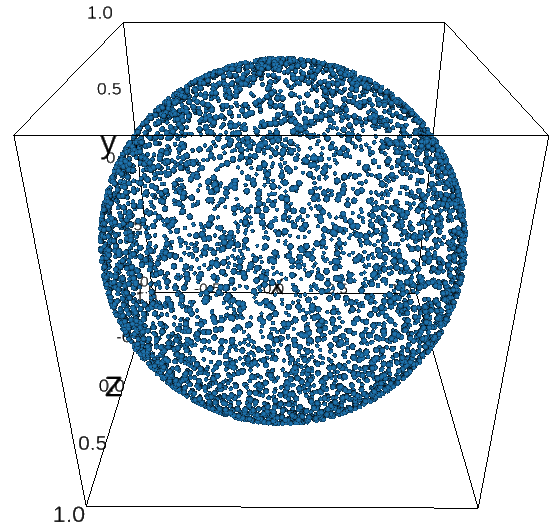
\includegraphics[height=7em]{figures/uniform_quaternion.png}%
        \hspace{1em}%
        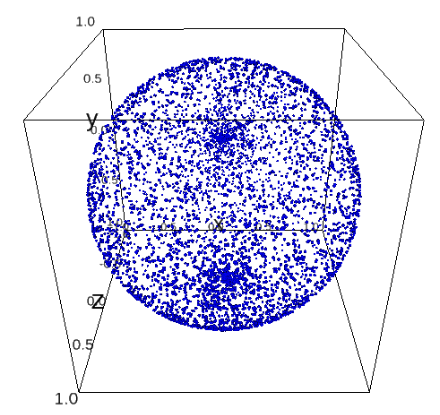
\includegraphics[height=7em]{figures/uniform_angles.png}
        \caption{Directions $(\theta_2, \theta_1)$ sampled uniformly from $\SO(3)$ (left) and Euler angles (right).}
    \end{subfigure}
    \hspace{4em}
    \begin{subfigure}[b]{0.46\linewidth}
        \centering
        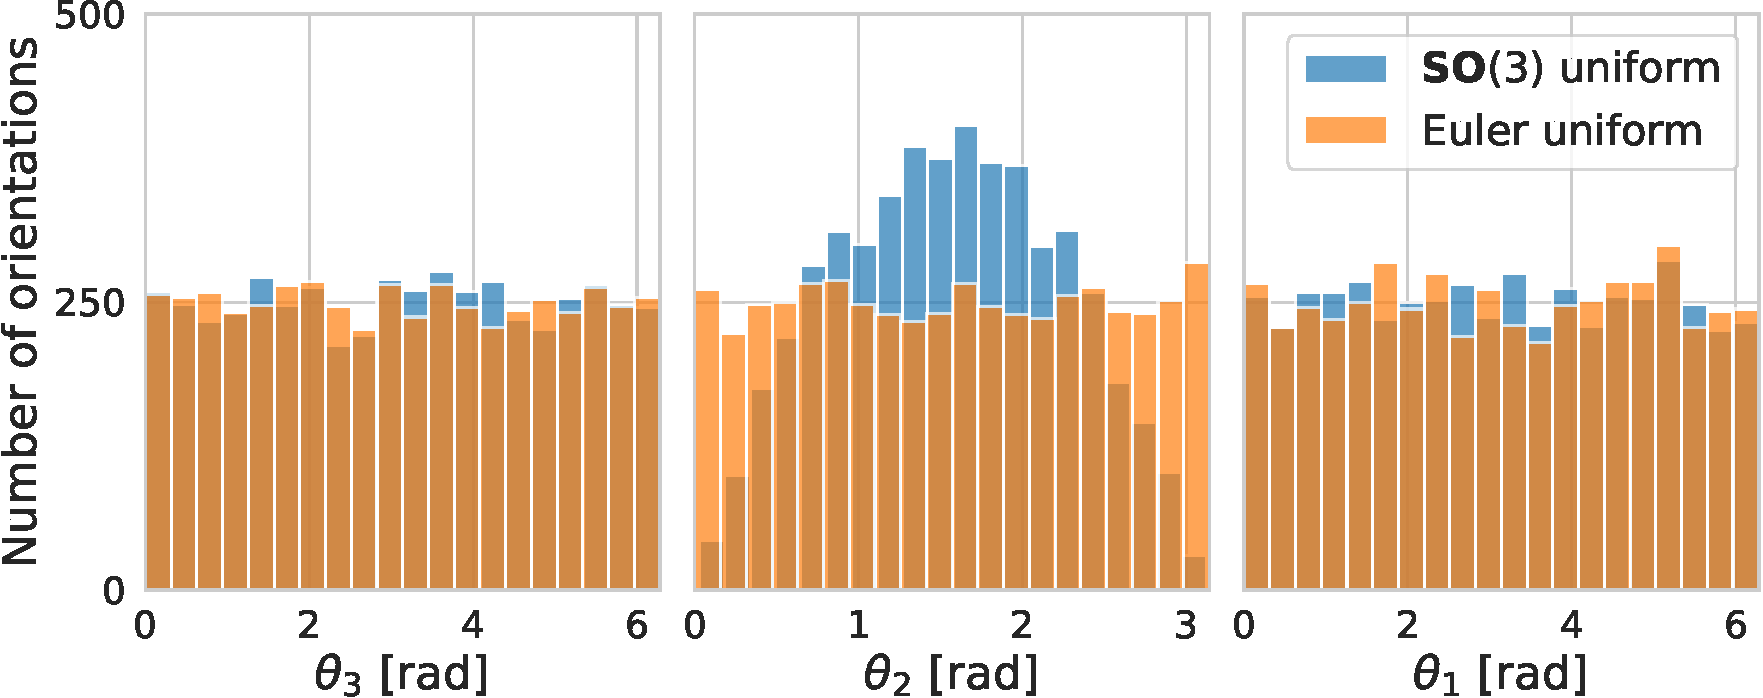
\includegraphics[height=8em]{figures/uniform_quaternions_vs_angles_ang.pdf}
        \caption{Distribution of Euler angles $\bth = (\theta_3,\theta_2,\theta_1)$.}
    \end{subfigure}
    \\ \vspace{1em}
    \begin{subfigure}[b]{0.36\linewidth}
        \centering
        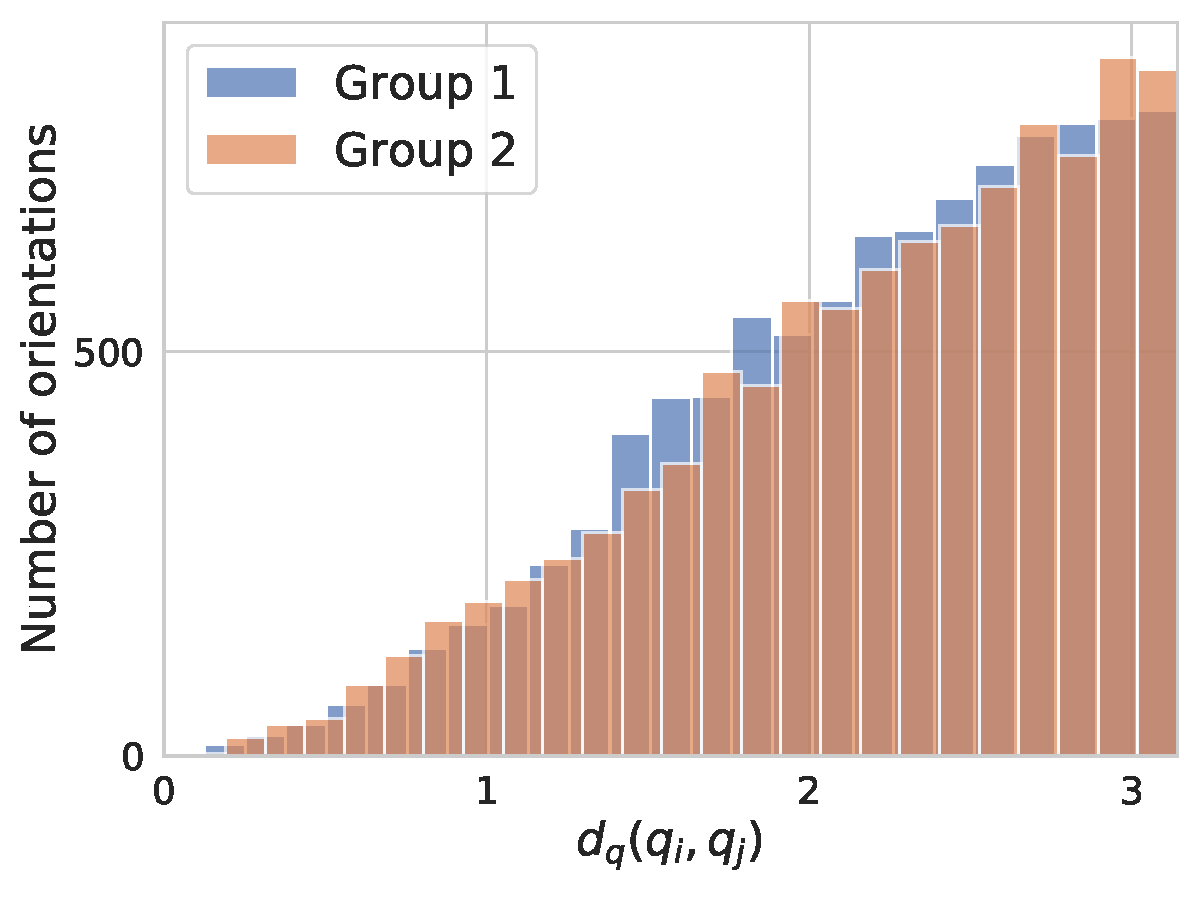
\includegraphics[height=8em]{figures/dQ_5j0n_uniform_quaternions_vs_angles.pdf}
        \caption{Distribution of ($10,000<P^2$) distances.}%
        \label{fig:orientation-sampling:distances}
    \end{subfigure}
    \hspace{1em}
    \begin{subfigure}[b]{0.46\linewidth}
        \centering
        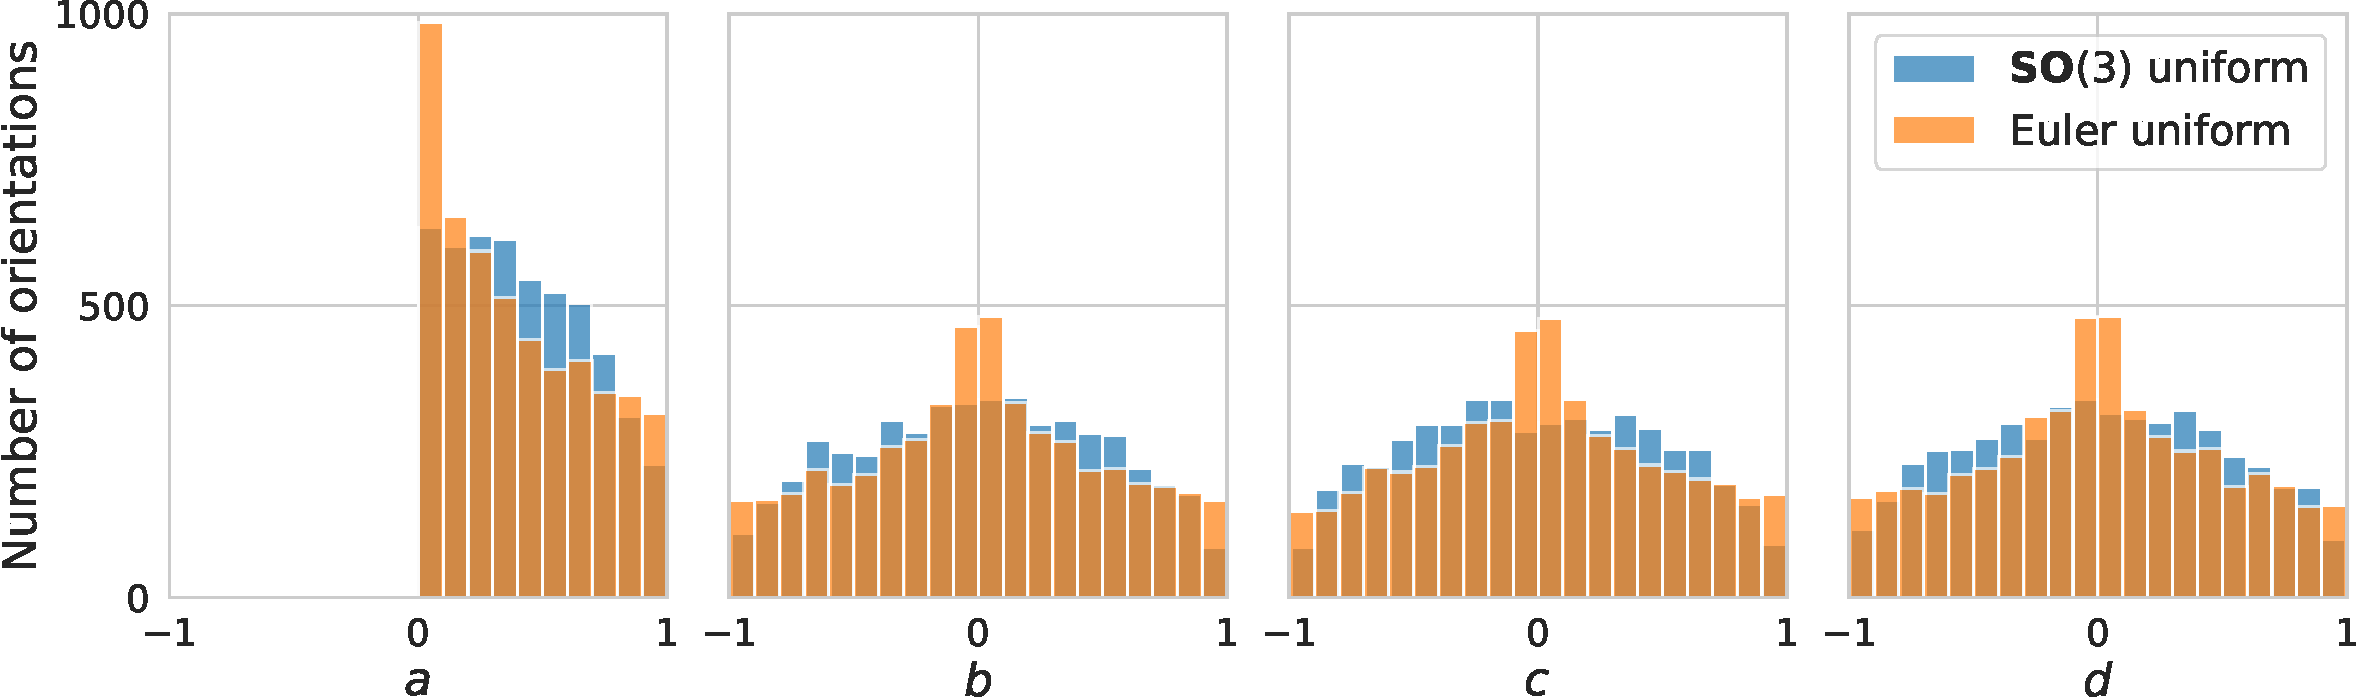
\includegraphics[height=8em]{figures/uniform_quaternions_vs_angles_q.pdf}
        \caption{Distribution of quaternions $q = a + b\boldsymbol{i} + c\boldsymbol{j} + d\boldsymbol{k}$.}
    \end{subfigure}
    \caption{%
        Uniform sampling of $P=5,000$ orientations from $\SO(3)$ (Group 1) and uniform sampling of $P=5,000$ Euler angles from $[0,2\pi[ \, \times \, [0,\pi] \times [0,2\pi[$ inducing a non-uniform distribution of orientations (Group 2).
        %\mdeff{That's not uniform in quaternion space, as shown by (d). ;) It's uniform in rotation / SO(3) space. How did you sample it? A classic way is to draw from $\mathcal{N}(0, I_4)$ then normalize to unit norm. More at \url{https://mathworld.wolfram.com/SpherePointPicking.html}.}\banjac{yes, we sample uniformly on SO(3), sorry my mistake in wording}
        %\todo{Legend with ``$\SO(3)$ uniform'' and ``Euler uniform'' rather than ``Group 1'' and ``Group 2''.}
    }\label{fig:orientation-sampling}
\end{figure}

\figref{orientation-constraints} shows distributions of induced distances when directions $(\theta_2, \theta_1)$ are constrained to an half or a quarter of the 2-sphere.
% (to learn from asymmetric proteins like \texttt{5j0n})
% (\eg, for proteins with D2 symmetry like \texttt{5a1a})
While the distributions flatten (compare with \figref{orientation-sampling:distances}), the shorter distances are still way under-sampled.

\begin{figure}[ht!]
    \centering
    \begin{subfigure}[t]{0.32\linewidth}
        \centering
        %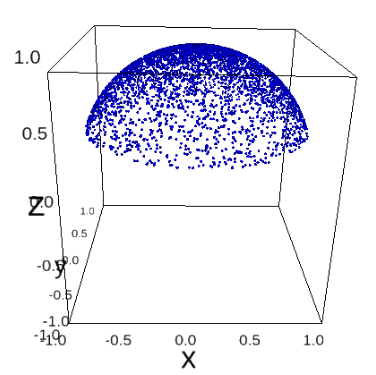
\includegraphics[height=7em]{figures/5j0n-half.png}
        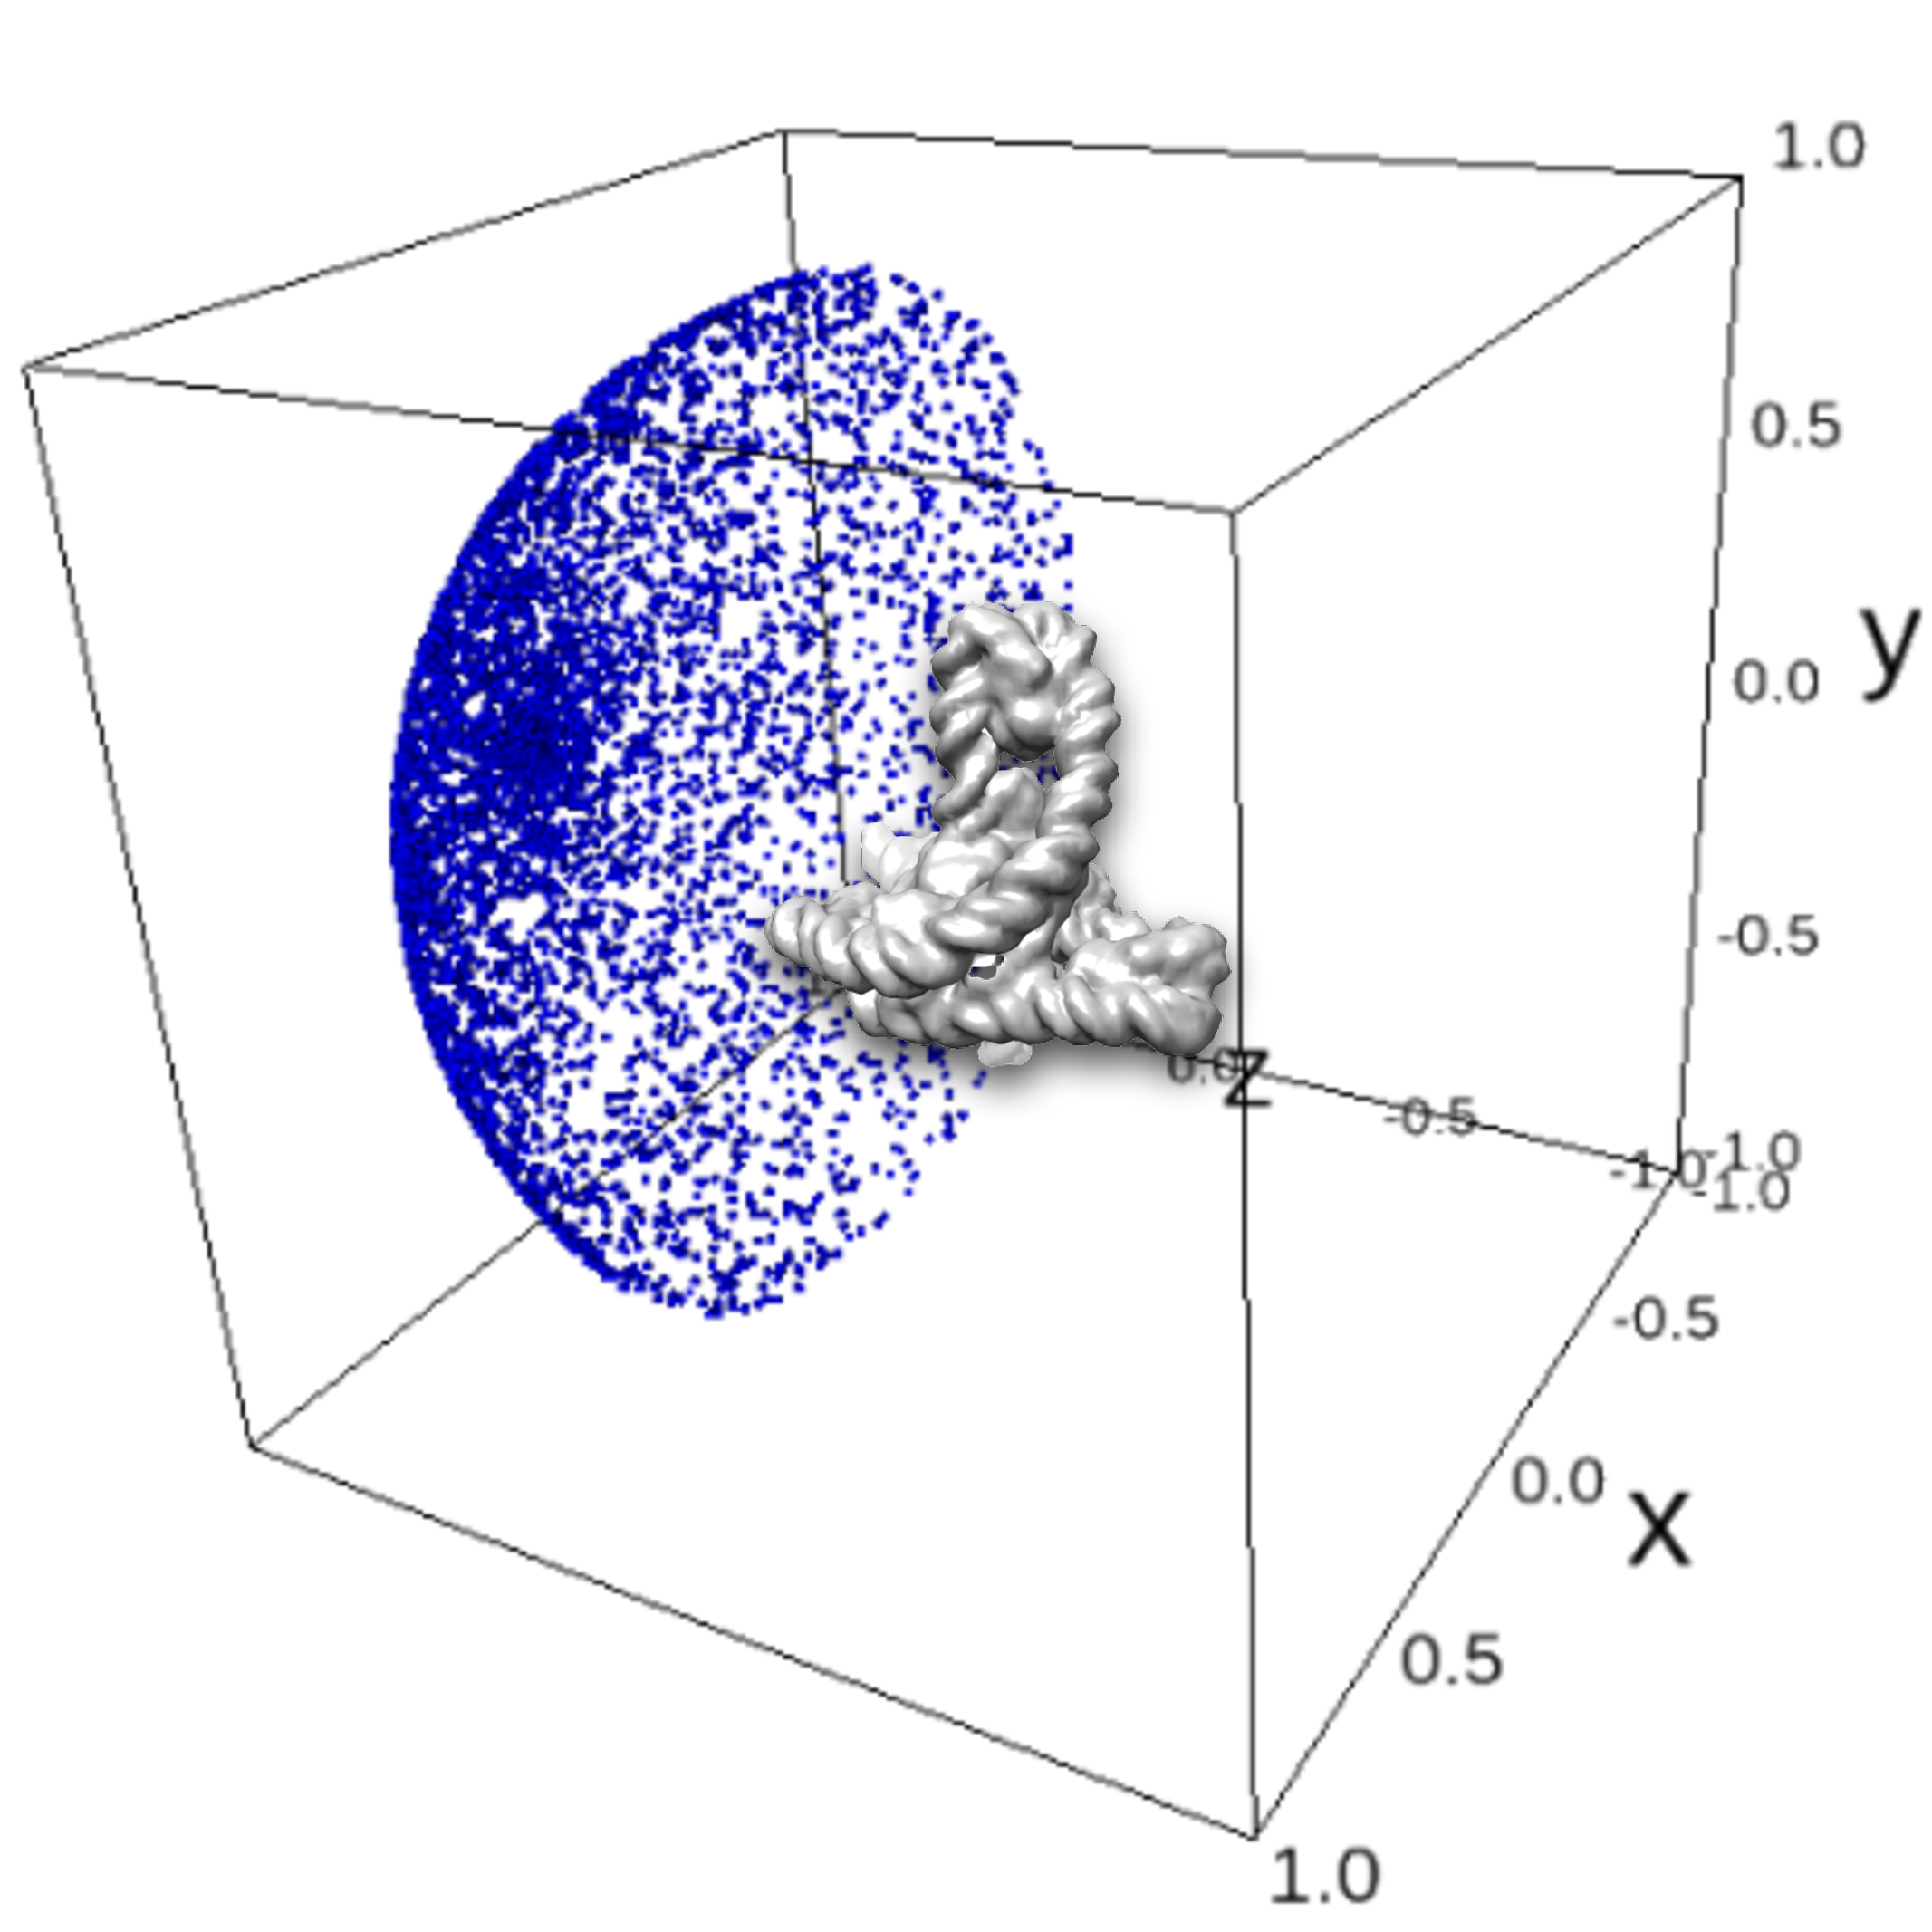
\includegraphics[height=9em]{figures/5j0n-cvg.pdf}
        \caption{Directions sampled from $(\theta_2, \theta_1) \in [0,\frac{\pi}{2}[ \, \times \, [0,2\pi[$, an half of the sphere.}
    \end{subfigure}
    \hfill
    \begin{subfigure}[t]{0.32\linewidth}
        \centering
        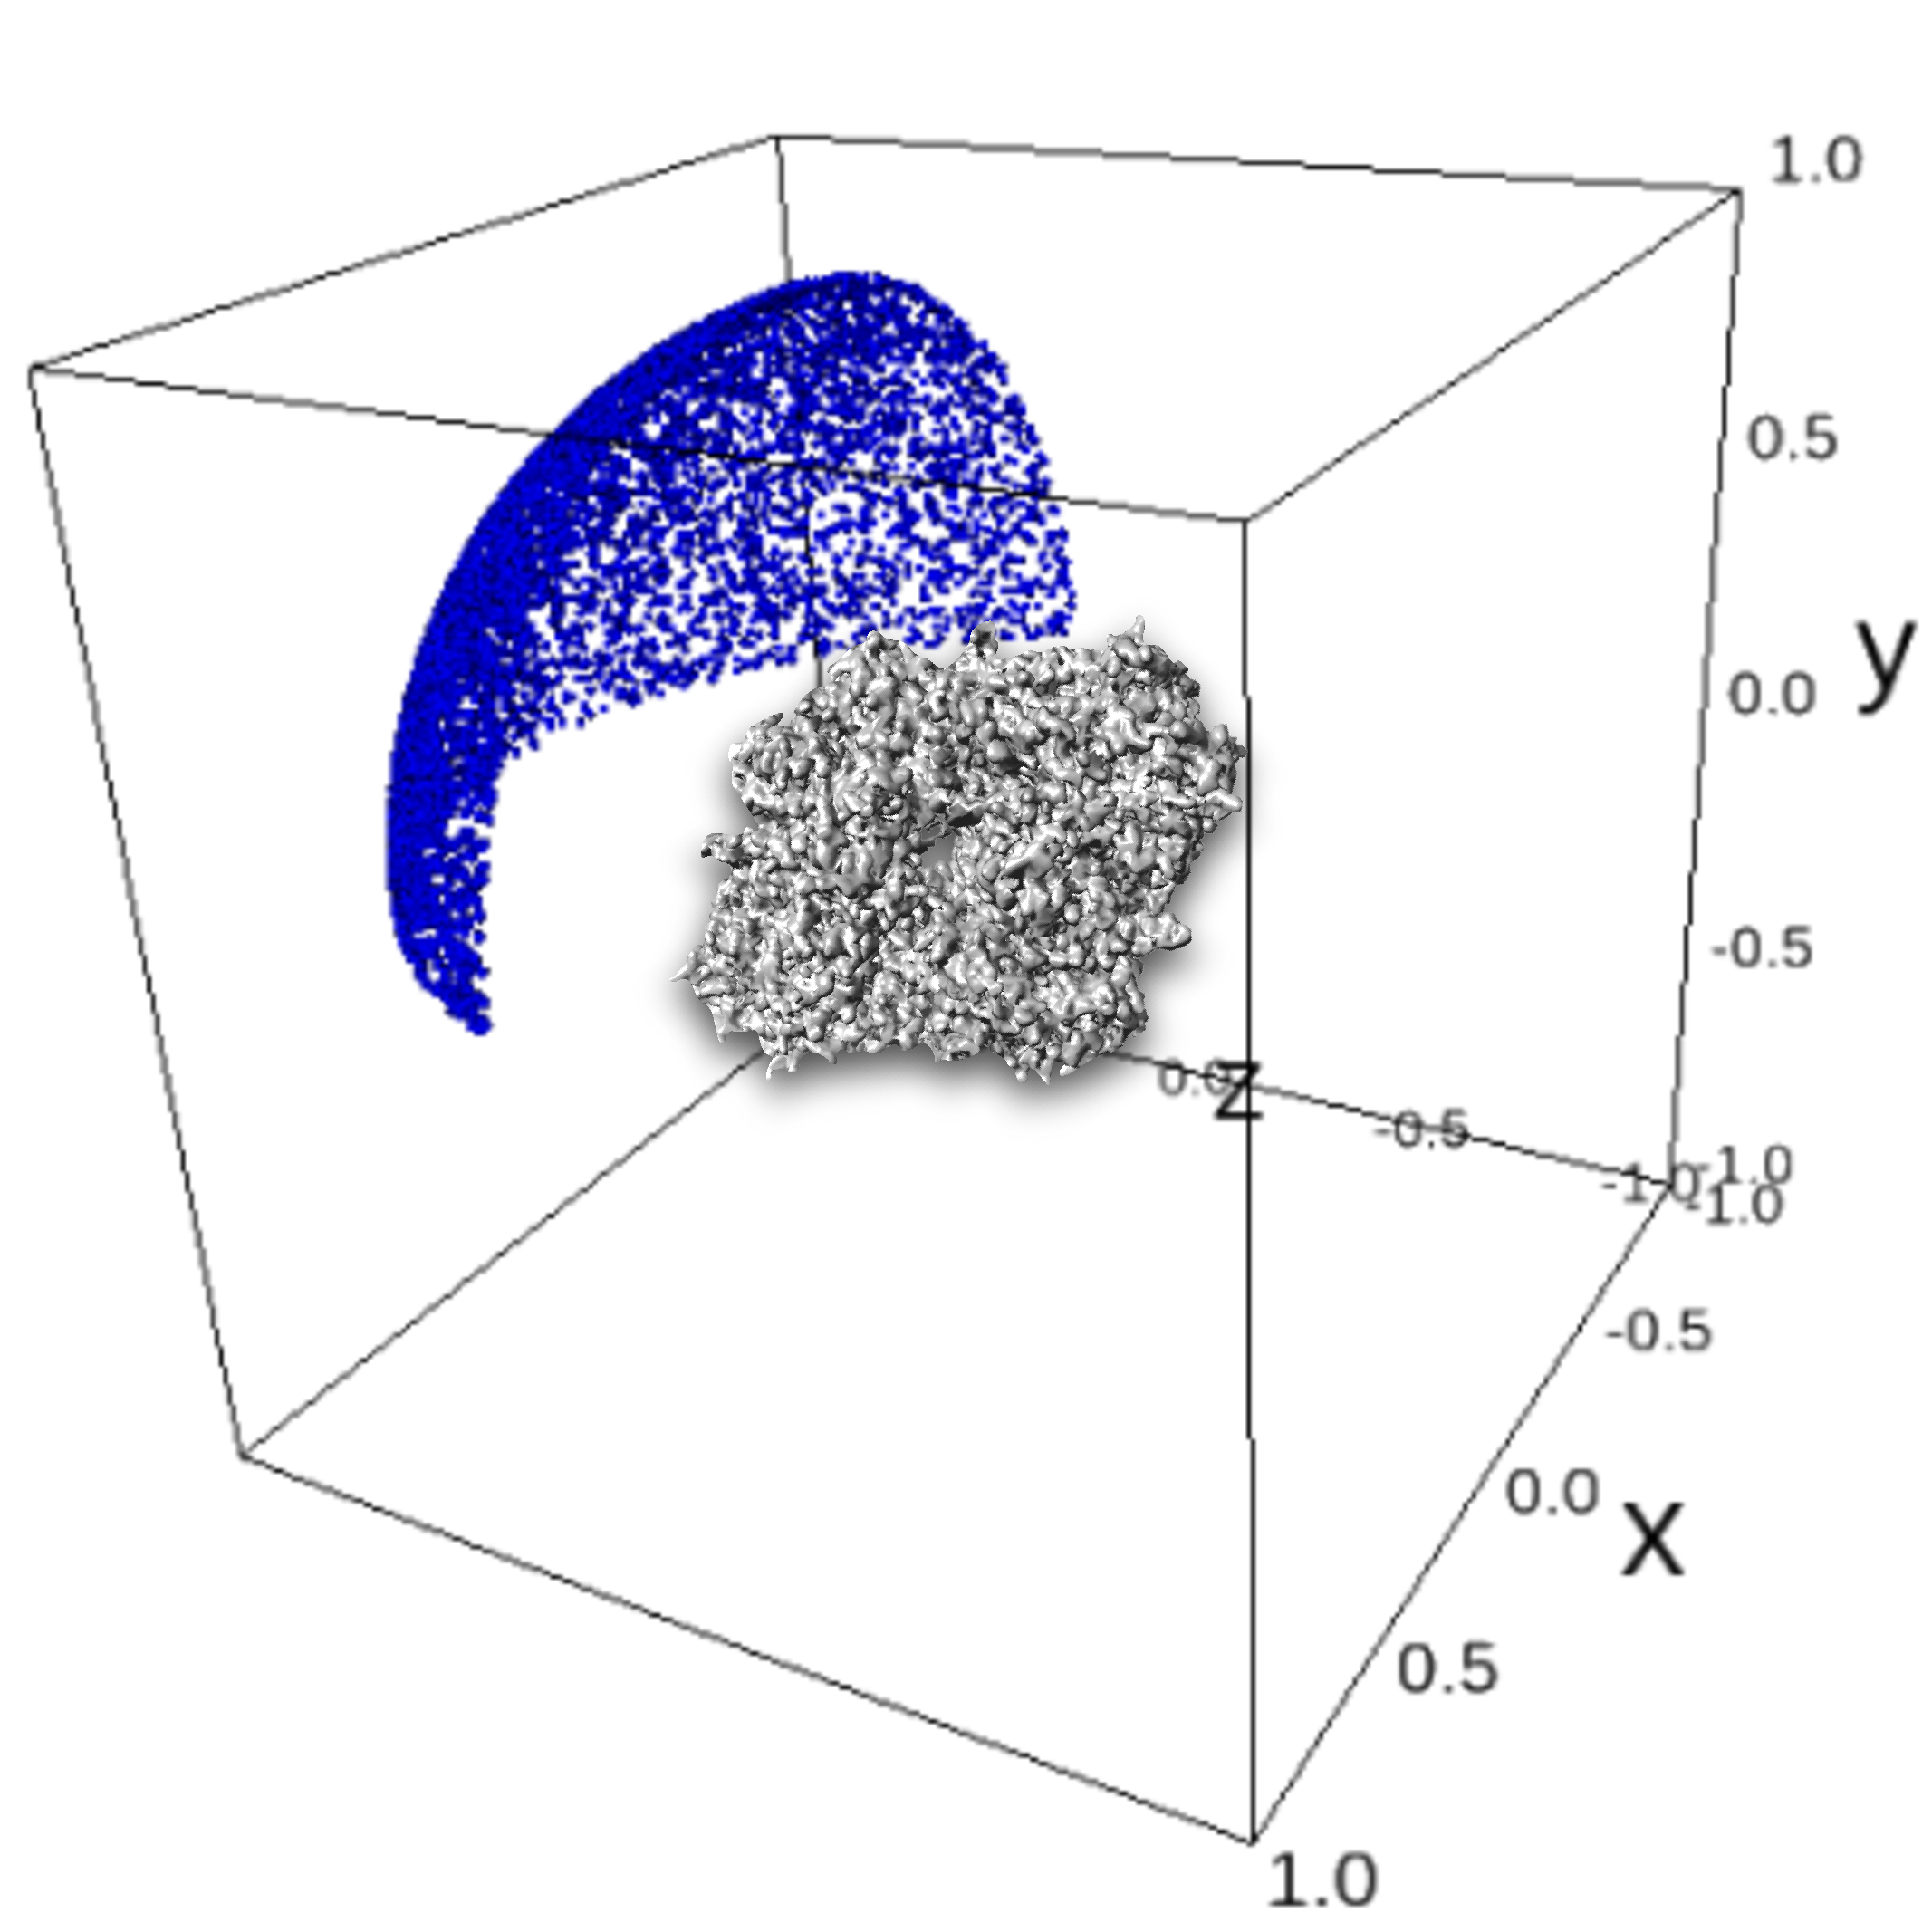
\includegraphics[height=9em]{figures/5a1a-cvg.pdf}
        \caption{Directions sampled from $(\theta_2, \theta_1) \in [0,\frac{\pi}{2}[ \, \times \, [0,\pi[$, a quarter of the sphere.}
    \end{subfigure}
    \hfill
    \begin{subfigure}[t]{0.32\linewidth}
        \centering
        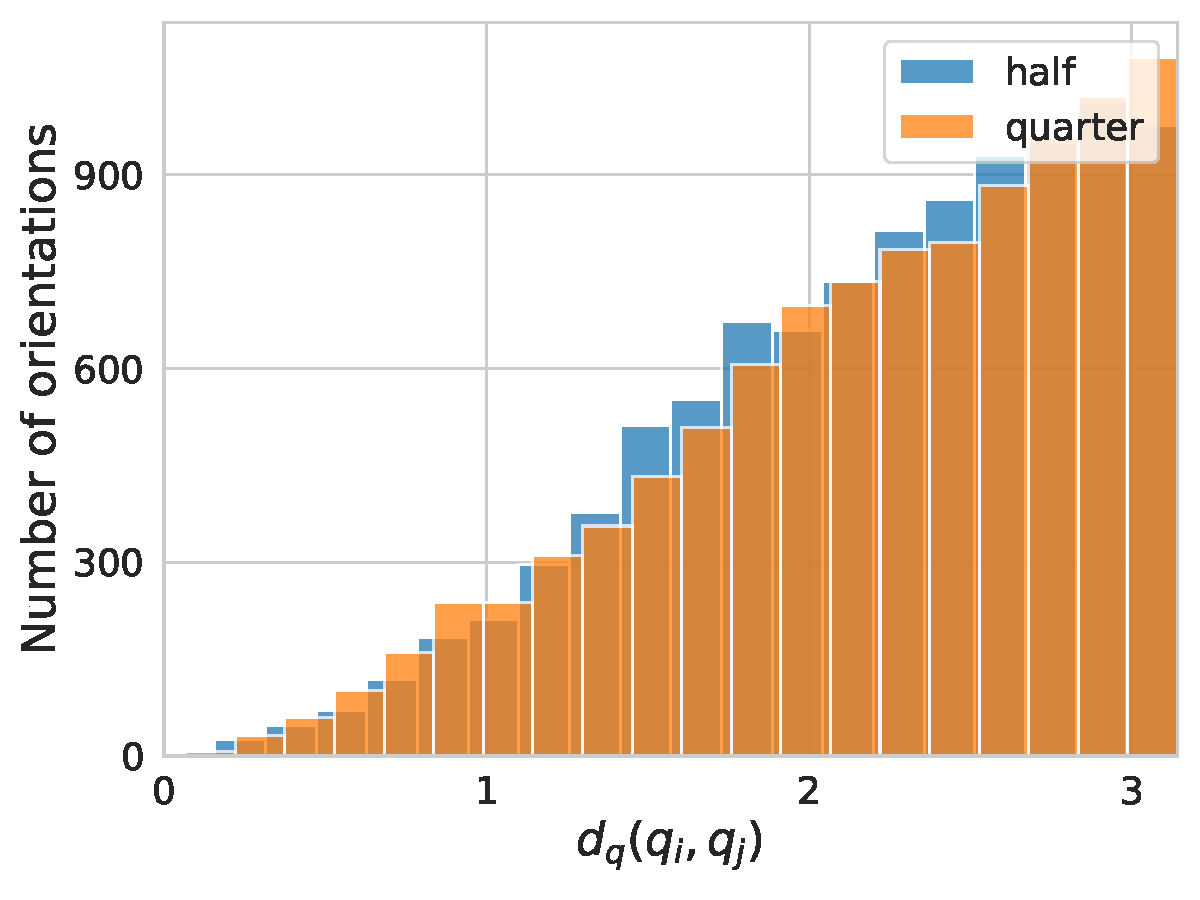
\includegraphics[height=9em]{figures/dQ_half_vs_quarter.pdf}
        \caption{Induced distribution of distances.}%
        \label{fig:orientation-constraints:distances}
    \end{subfigure}
    \caption{%
        Distributions of $P=5,000$ directions $(\theta_2, \theta_1)$ as points on the sphere (see also \figref{imaging-geometry}), illustrating their constrained range, and the distances they induce.
    }\label{fig:orientation-constraints}
\end{figure}

\begin{figure}[ht!]
    \centering
    \begin{subfigure}[b]{0.60\linewidth}
        \centering
        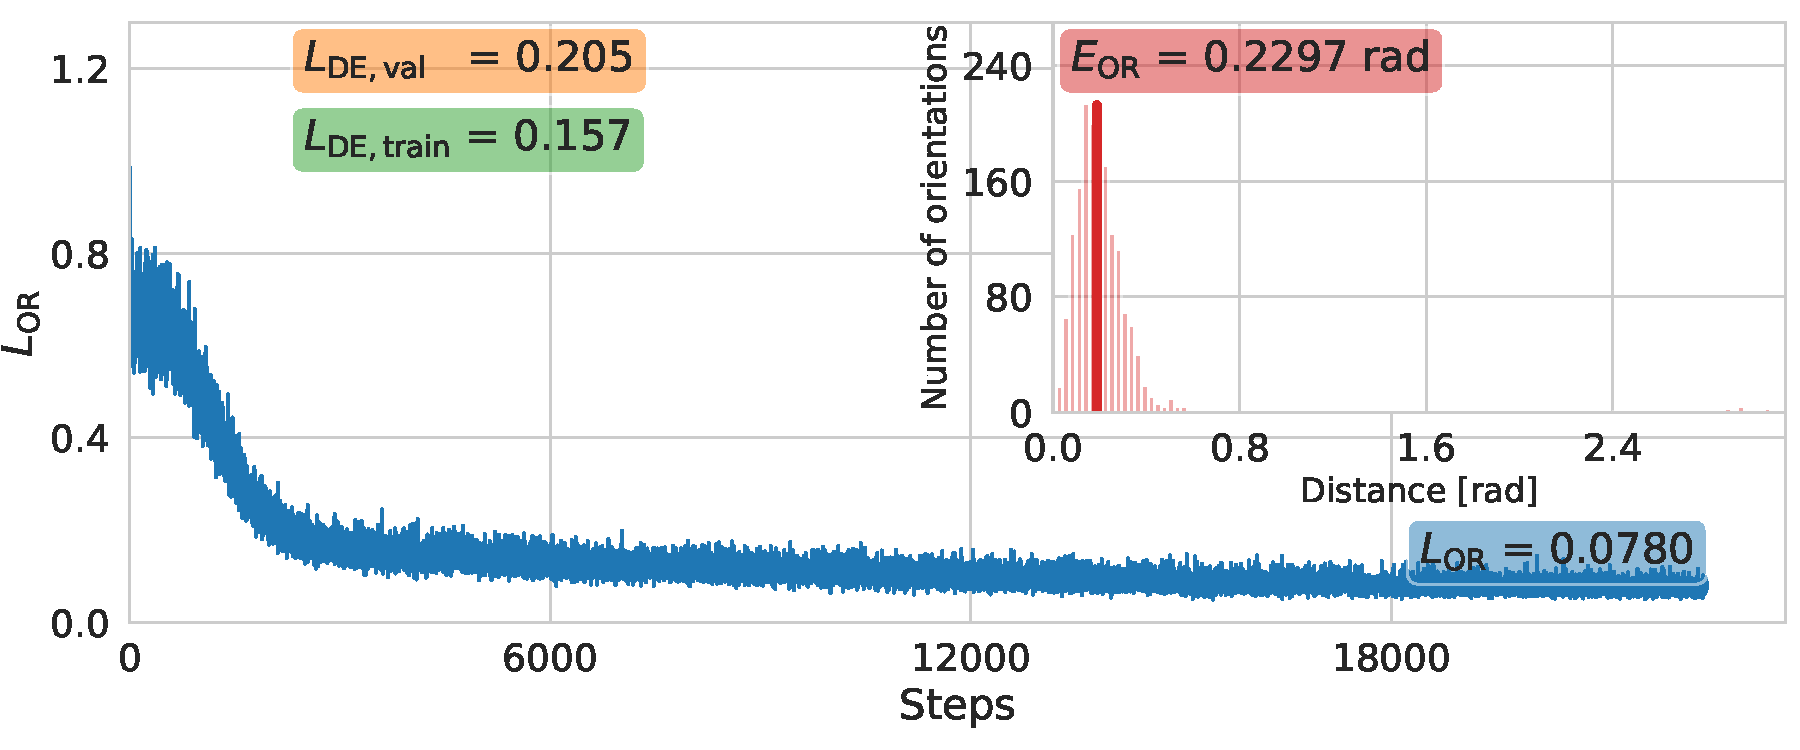
\includegraphics[height=4cm]{figures/5j0n_ar_aa_fullcvg.pdf}
        \caption{Recovered $\{ \widehat{q_i} \}$ from noiseless \texttt{5j0n} projections $\{ \p_i \}$.}
    \end{subfigure}
    \hfill
    \begin{subfigure}[b]{0.38\linewidth}
        \centering
        % 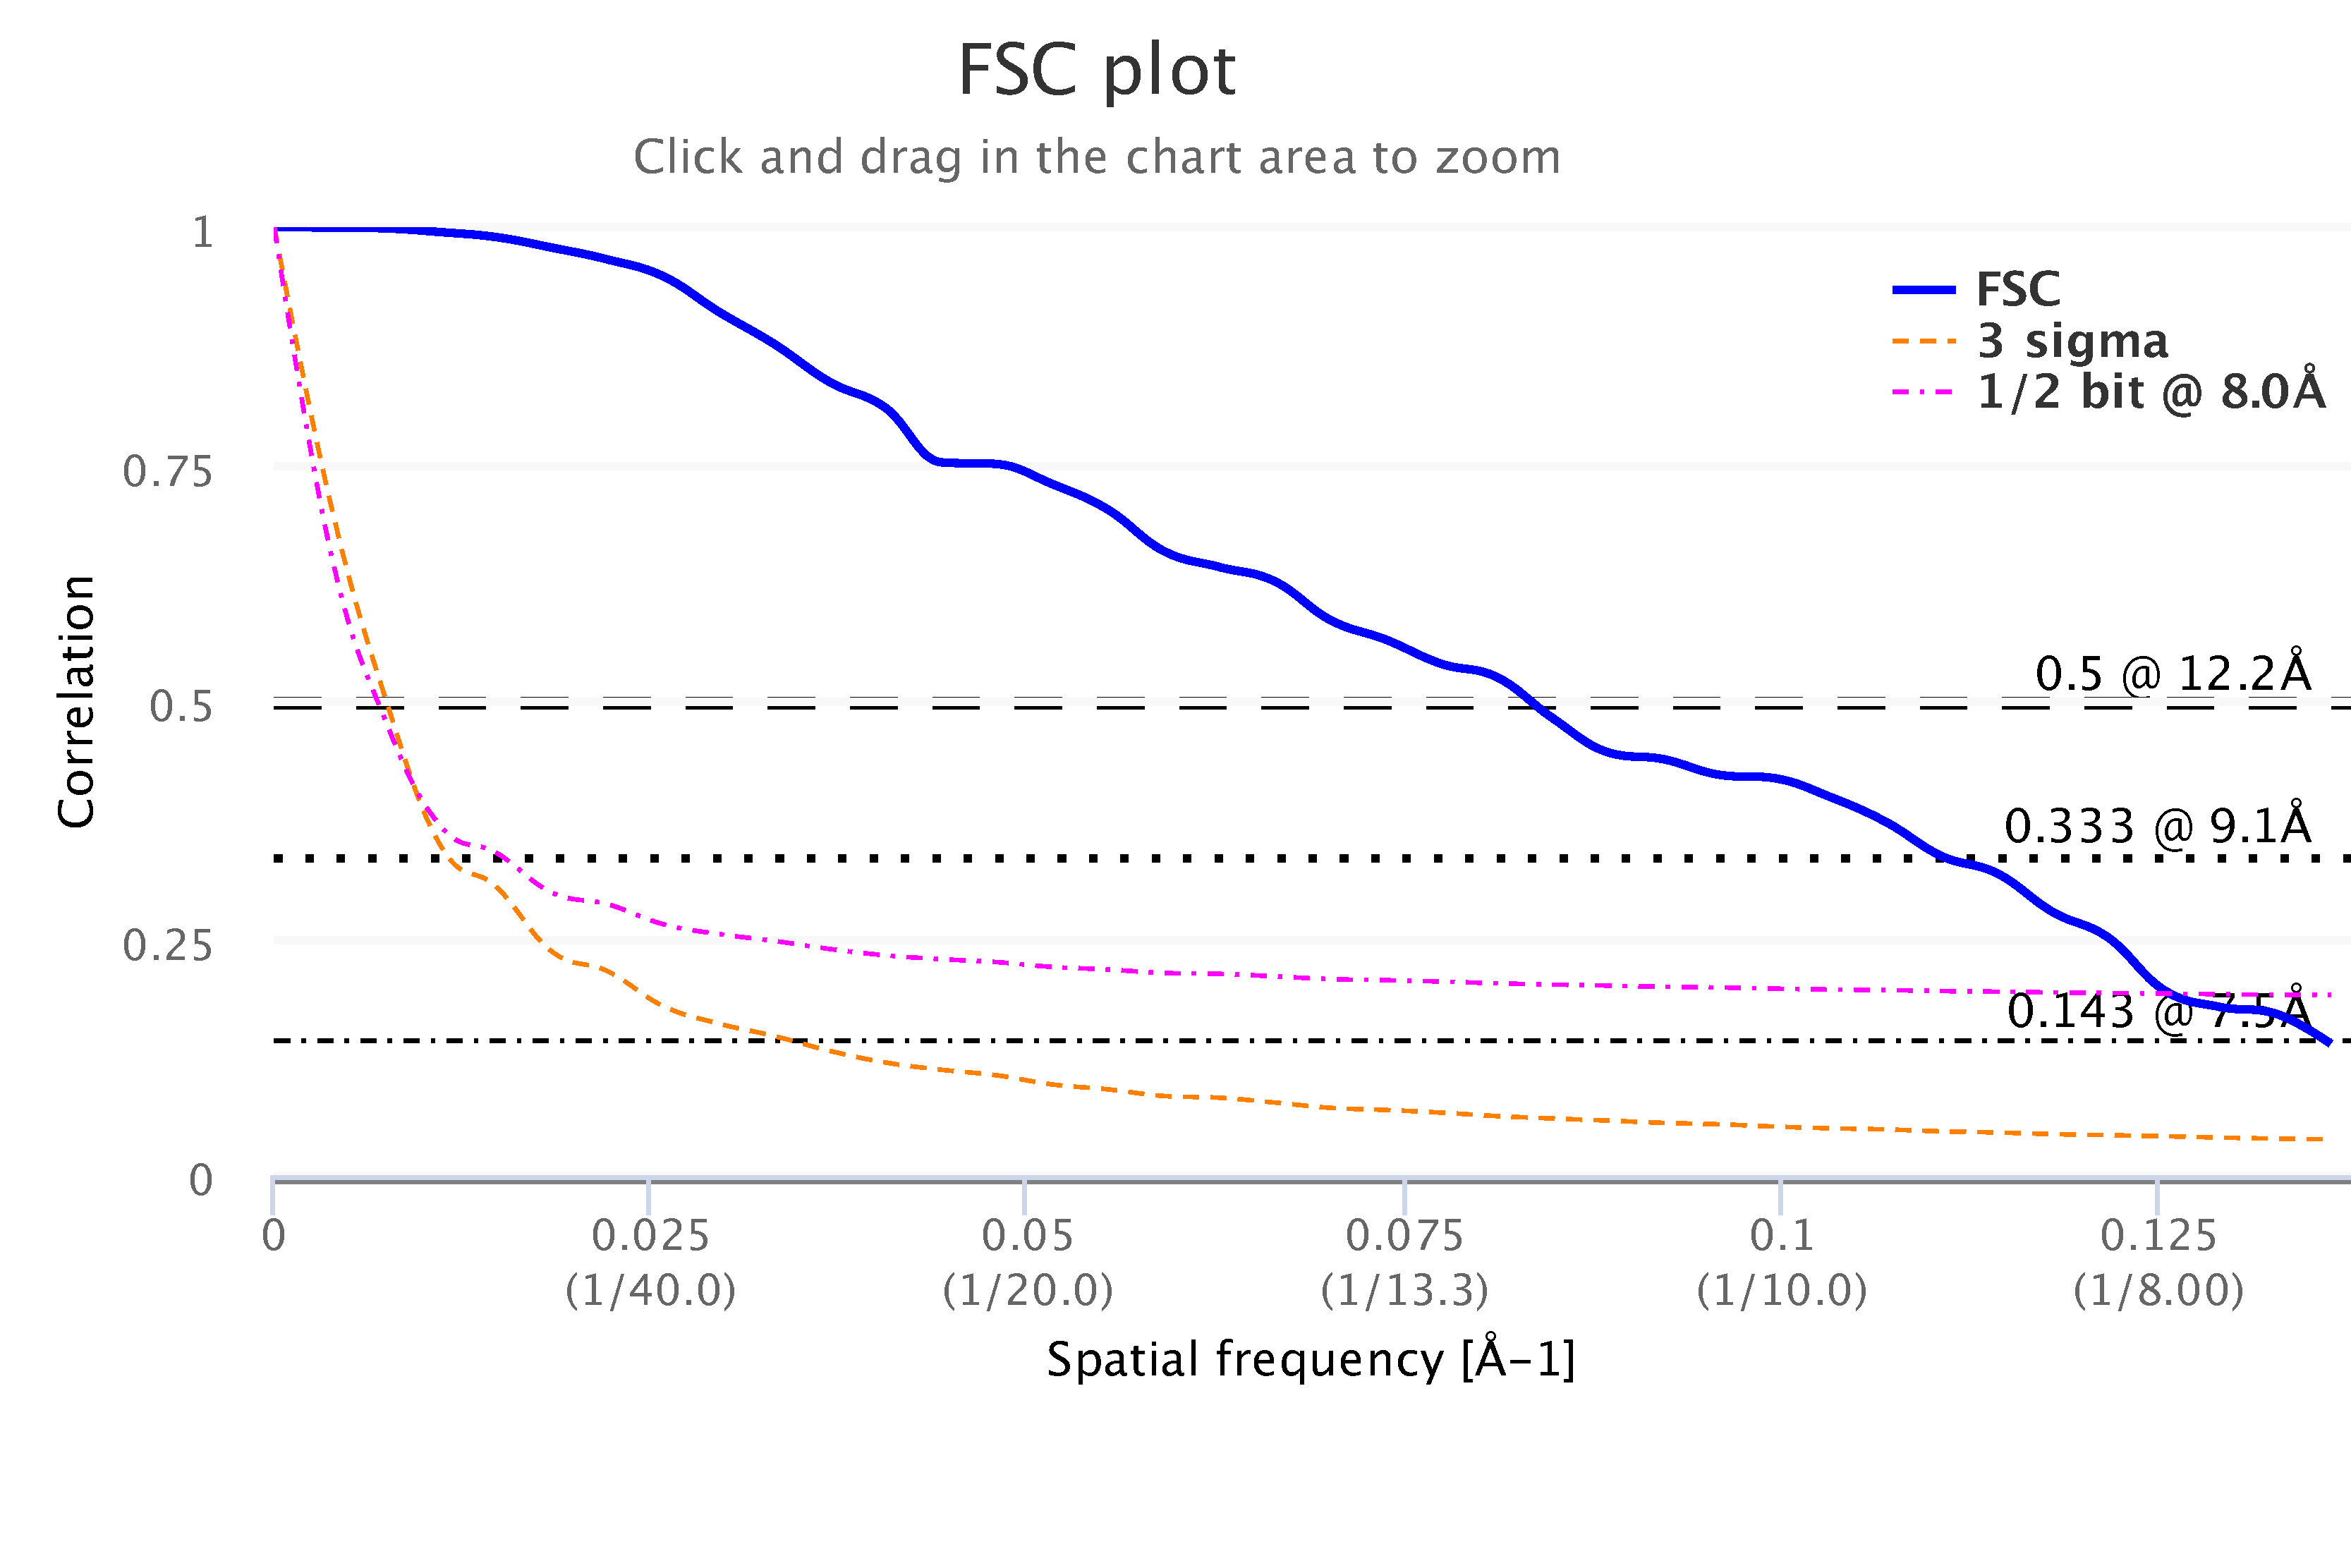
\includegraphics[height=4cm]{figures/FSC_5j0n_fullcvg_noise0_fin_vs_init.pdf}
        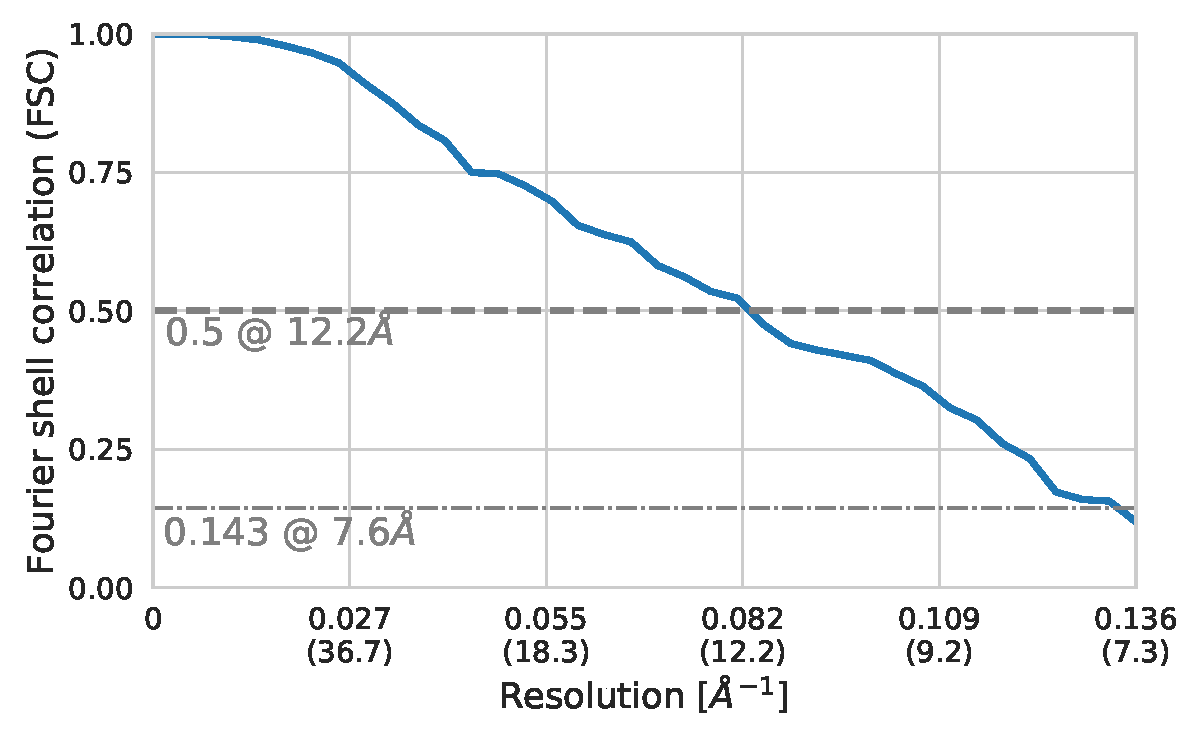
\includegraphics[height=4cm]{figures/5j0n_fullcvg_noise0_FSC_apr_init_customFSC.pdf}
        
        \caption{Fourier shell correlation of the reconstruction.}
    \end{subfigure}
    \caption{%
        Orientation recovery and density reconstruction from projections acquired from non-uniformly orientations (uniformly sampled Euler angles).
        %Full pipeline on the orientations with uniform sampling of Euler angles from full 2-sphere coverage.
        %\todo{Update the FSC plot as in \figref{reconstructions}.}
    }\label{fig:recovery-nonuniform}
\end{figure}

\section{Orientation recovery from exact distances}\label{apx:results:orientation-recovery:exact}

%\mdeff{Story: works perfectly despite no convexity guarantee and sampling.}

\lau{Smooth.}
To verify that the lack of a convexity guarantee for \eqnref{orientation-recovery} and the sampling of the sum are non-issues in practice, we attempted orientation recovery under exact distance estimation $d_p(\p_i, \p_j) = d_q(q_i, q_j)$.
Orientations were perfectly recovered.
\figref{5j0n-orientation-recovery-loss} shows the convergence of the loss $L_\text{OR}$ to zero.
\figref{5j0n-aa-loss-perfect-distances} shows how~\eqnref{orientation-recovery-error} could then perfectly align the recovered and true orientations---leading to $E_\text{OR} = 0$.
% Demonstrating that alignment is necessary to evaluate the performance of orientation recovery.

\begin{figure}[ht!]
    \begin{minipage}[t]{0.39\linewidth}
        \centering
        %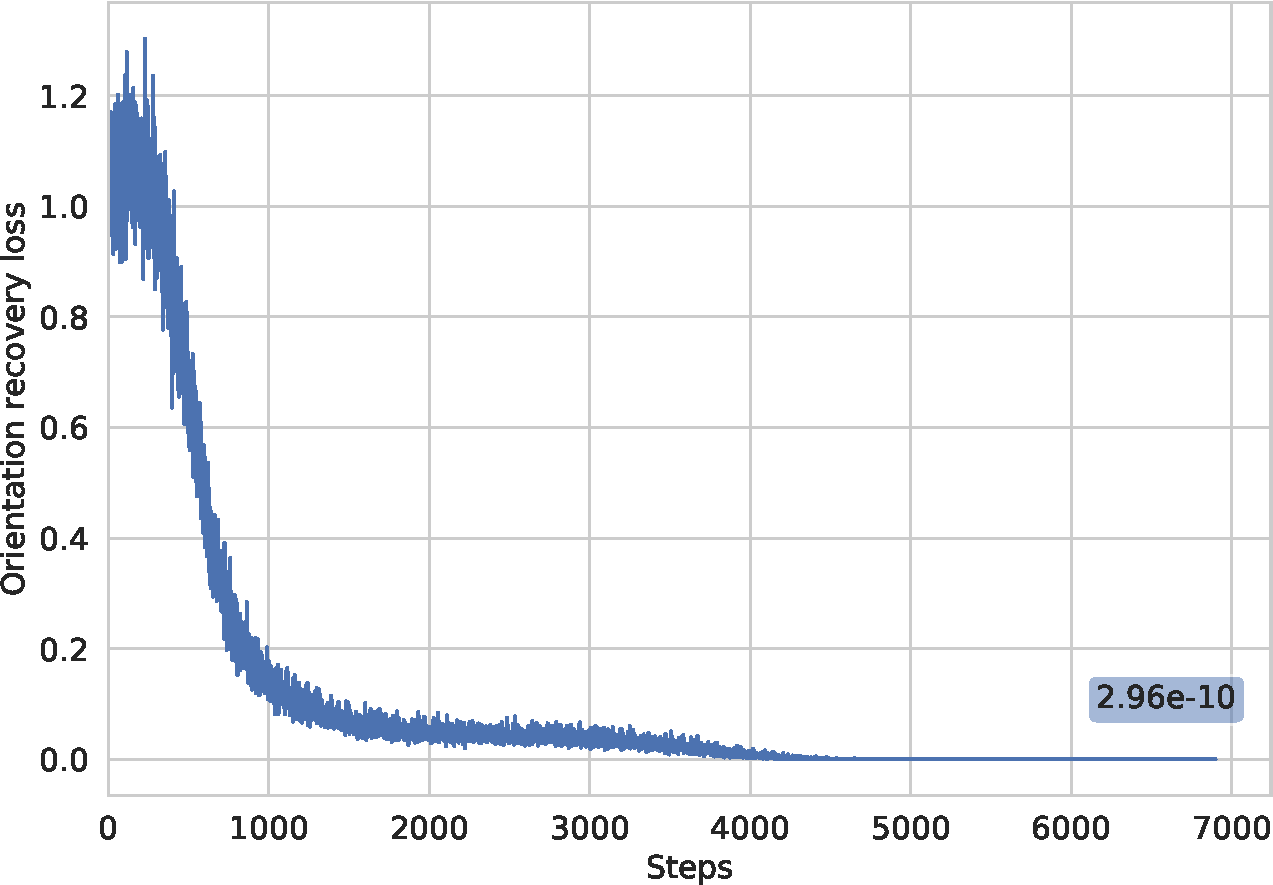
\includegraphics[height=3cm]{figures/5j0n_perfect_angle_recovery}
        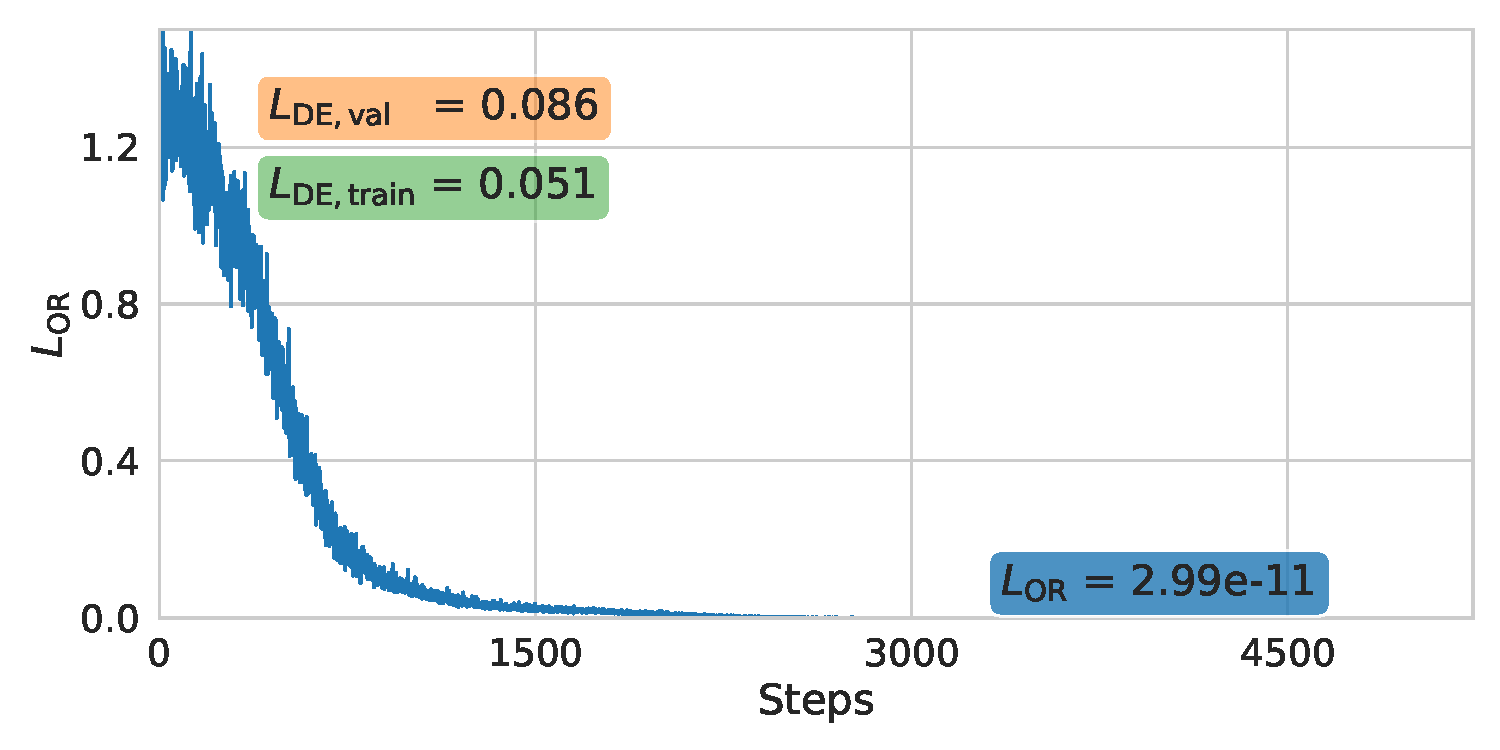
\includegraphics[height=3cm]{figures/5a1a_quartercov_uniformS2_halfInplane_ar_aa}
        \caption{%
            Example of perfect orientation recovery (for \texttt{5a1a}).
            The loss $L_\text{OR}$ \eqnref{orientation-recovery} converges to zero when the distance estimation is perfect, \ie, $\widehat{d_p}(\p_i, \p_j) = d_q(q_i, q_j)$.
            \todo{Update to full in-plane.}
        }\label{fig:5j0n-orientation-recovery-loss}
    \end{minipage}
    \hfill
    \begin{minipage}[t]{0.58\linewidth}
%        \begin{subfigure}[b]{0.19\linewidth}
%            \centering
%            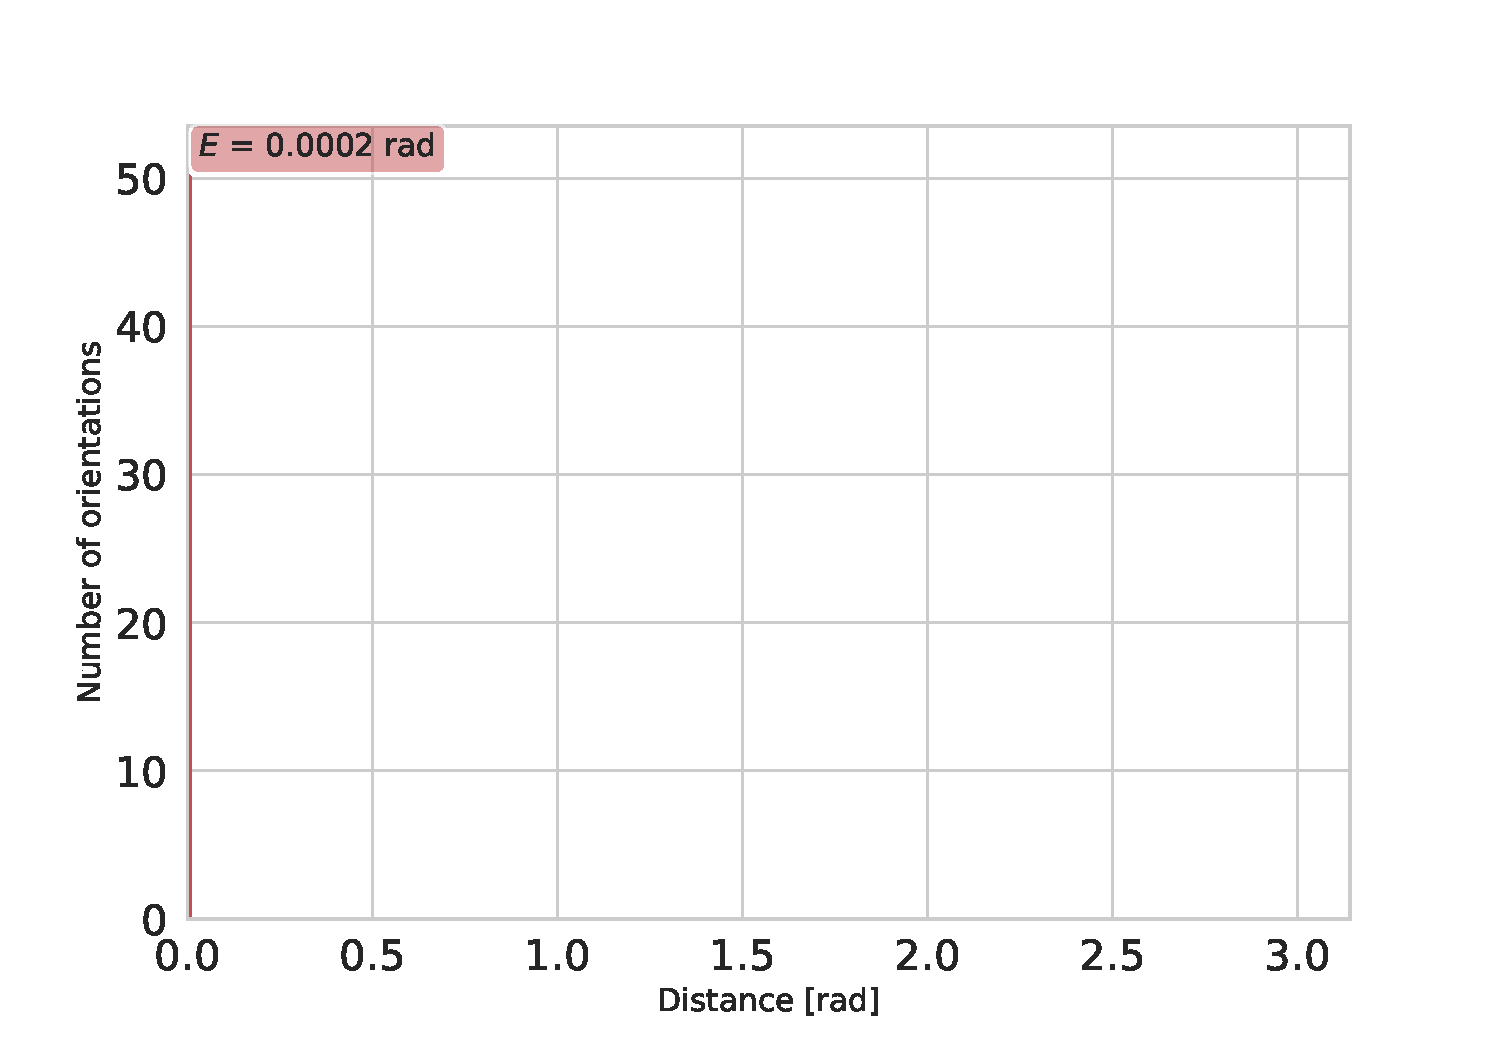
\includegraphics[height=3cm]{figures/5j0n_perfect_angle_ralignment_after}
%            \caption{Orientation recovery error with alignment.}
%        \end{subfigure}
%        \hfill
        % \begin{subfigure}[t]{4.3cm}
        %     \centering
        %     %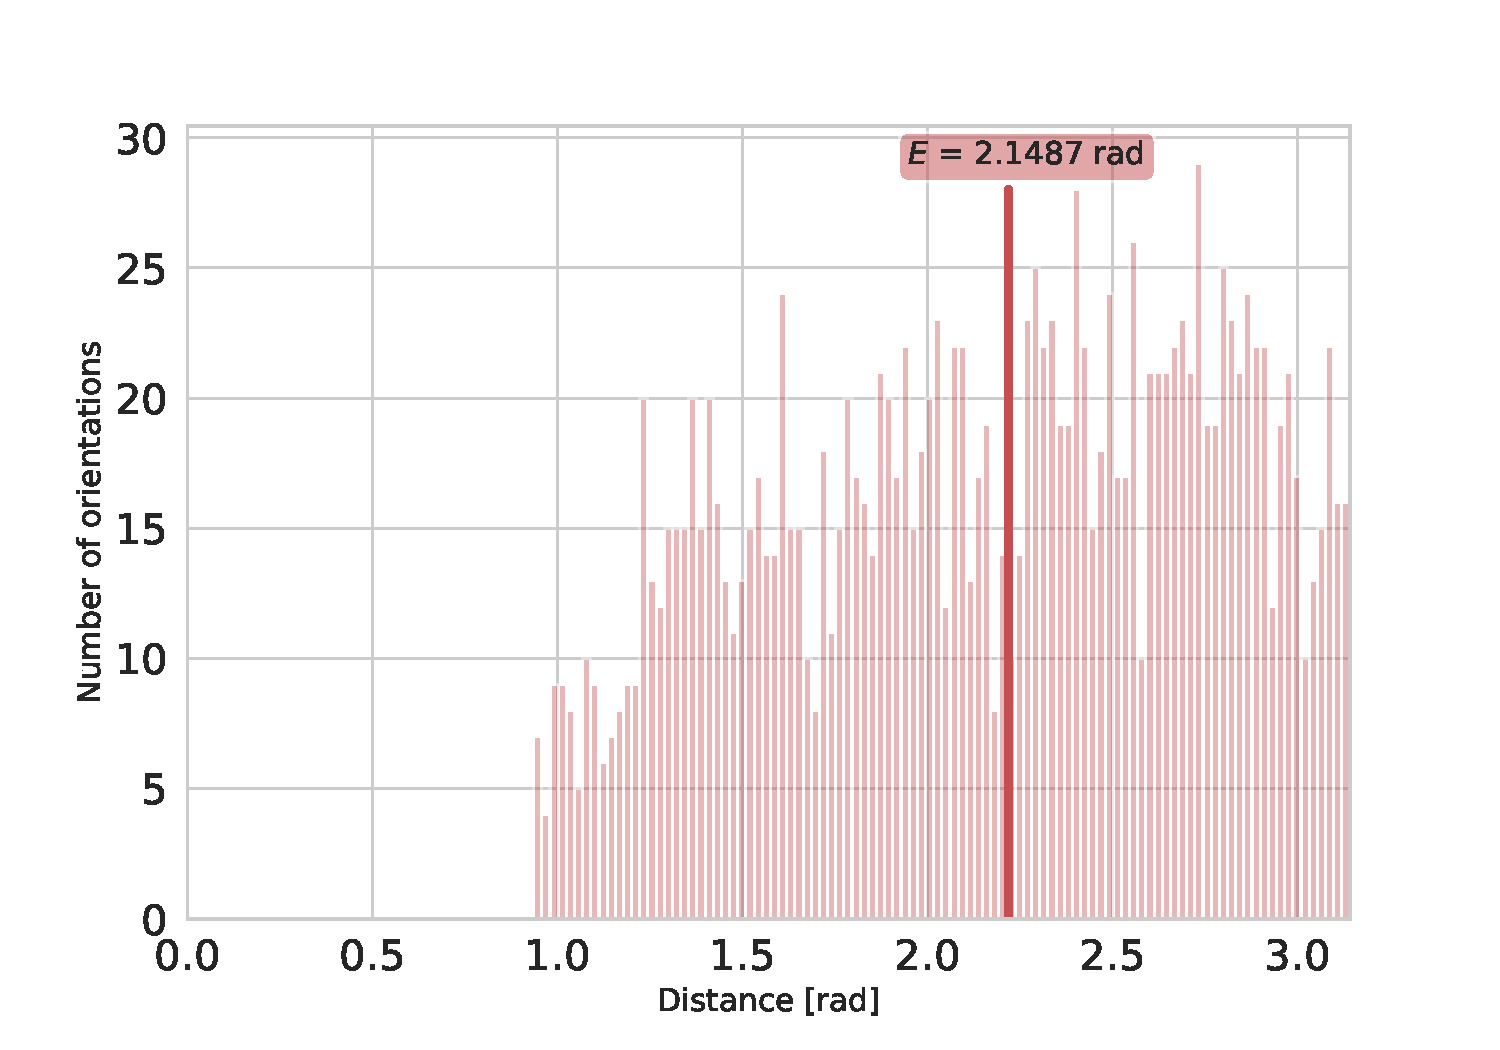
\includegraphics[height=3cm]{figures/5j0n_perfect_angle_ralignment_before}
        %     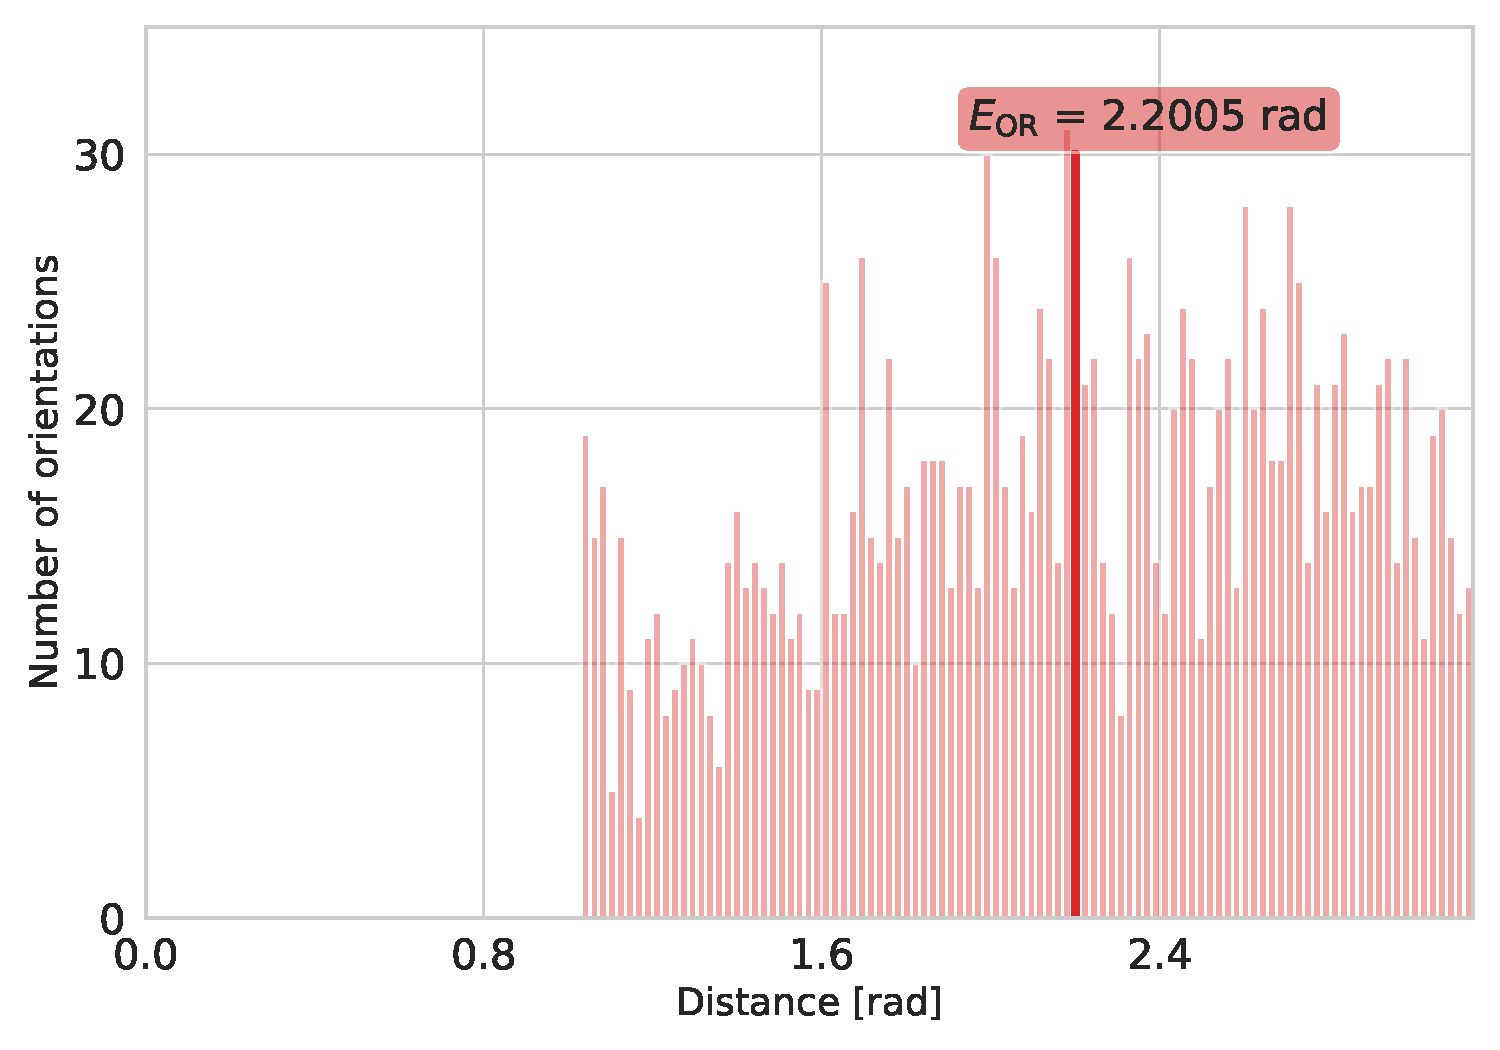
\includegraphics[height=3cm]{figures/5a1a_quartercov_uniformS2_halfInplane_before_alignment}
        %     \caption{Error histogram $\{ d_q (q_i, \widehat{q_i}) \}$, \ie, before alignment.}
        % \end{subfigure}
        % \hfill
        \begin{subfigure}[t]{0.47\linewidth}
            \centering
            % 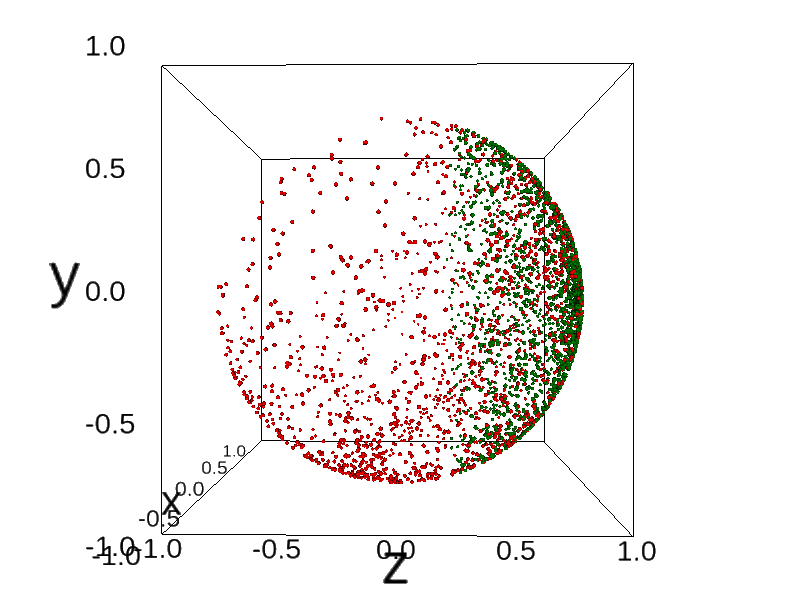
\includegraphics[height=3cm]{figures/coverage_alignment_before.png}
            %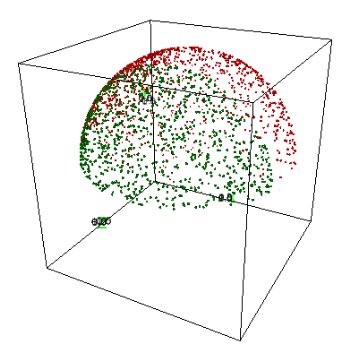
\includegraphics[height=3cm]{figures/before_aa.png}
            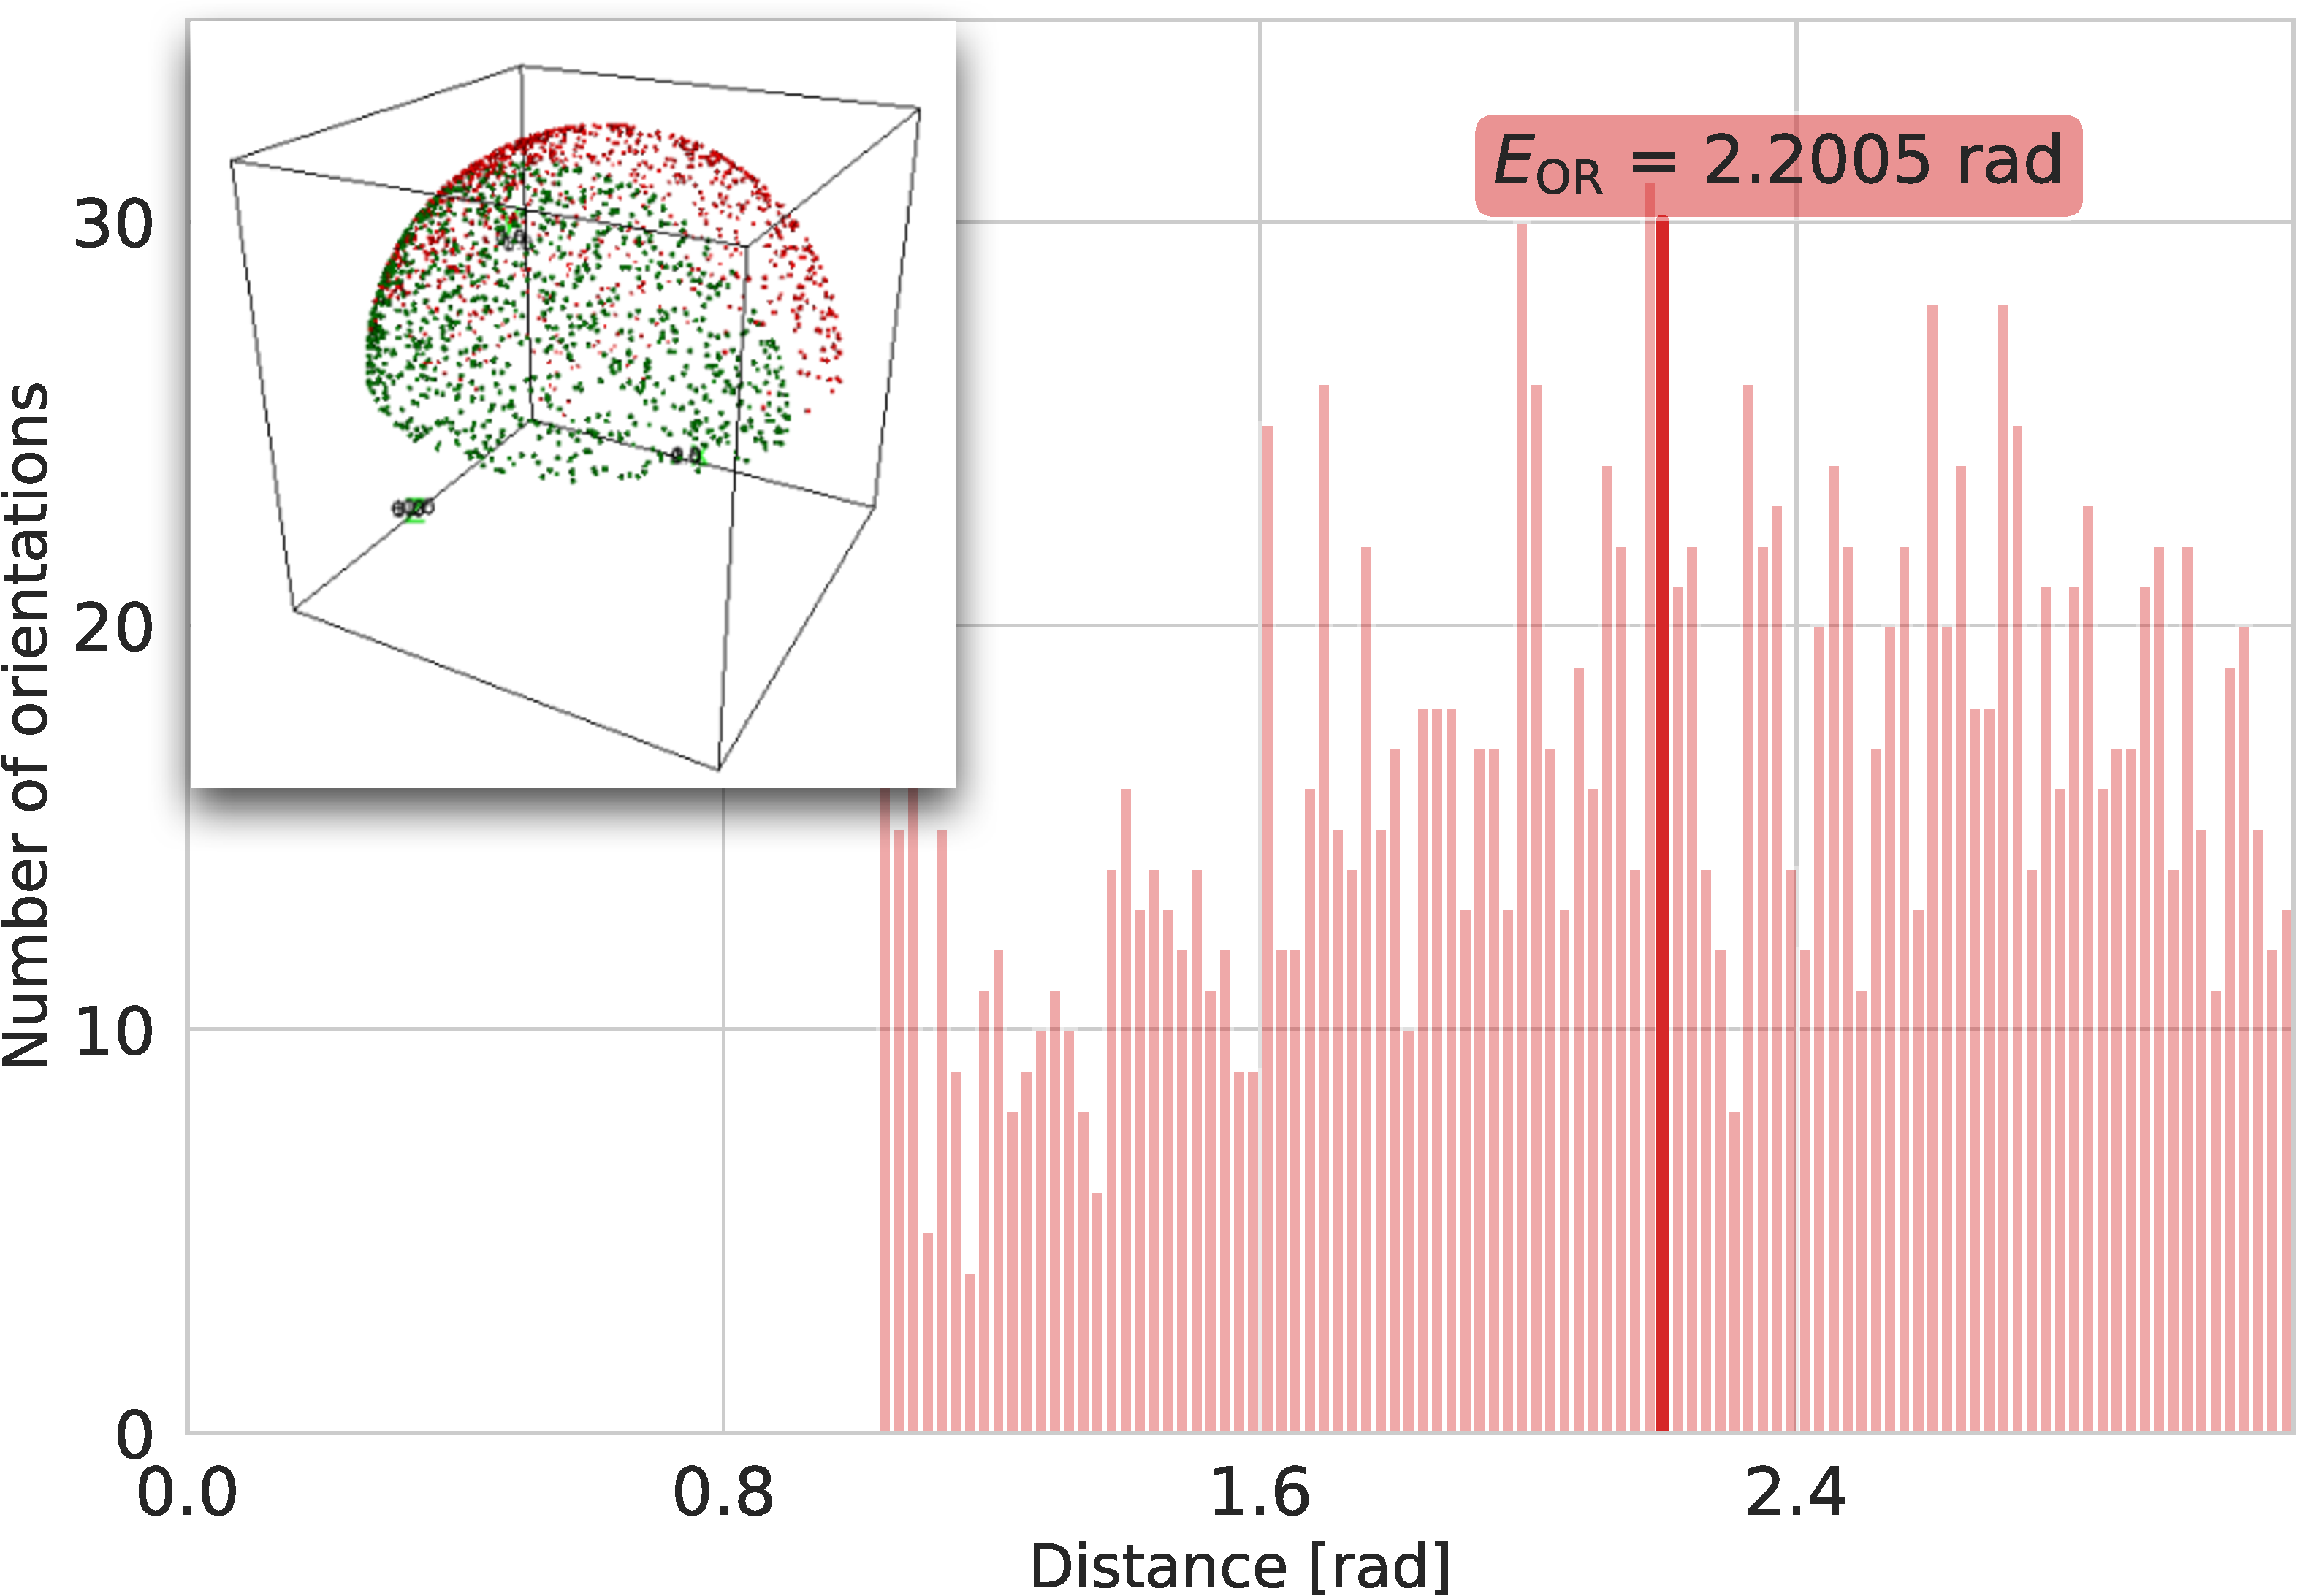
\includegraphics[height=3cm]{figures/BeforeAA.pdf}
            \caption{Orientations before alignment.}
        \end{subfigure}
        \hfill
        \begin{subfigure}[t]{0.47\linewidth}
            \centering
            % 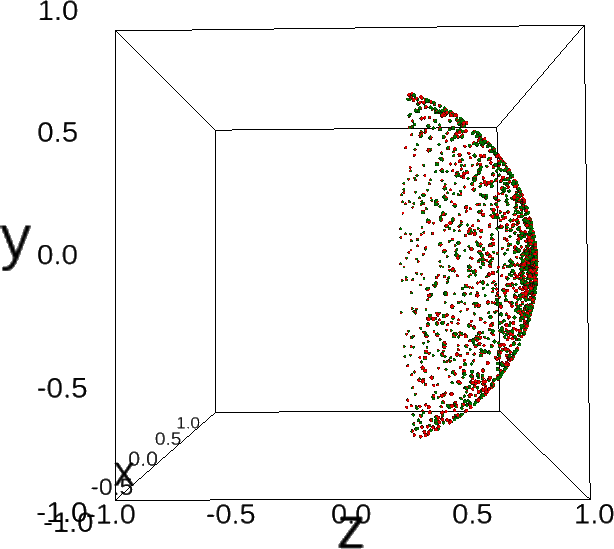
\includegraphics[height=3cm]{figures/coverage_alignment_after.png}
            %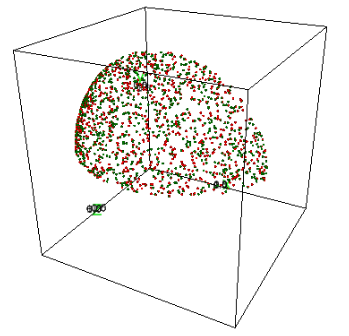
\includegraphics[height=3cm]{figures/after_aa.png}
            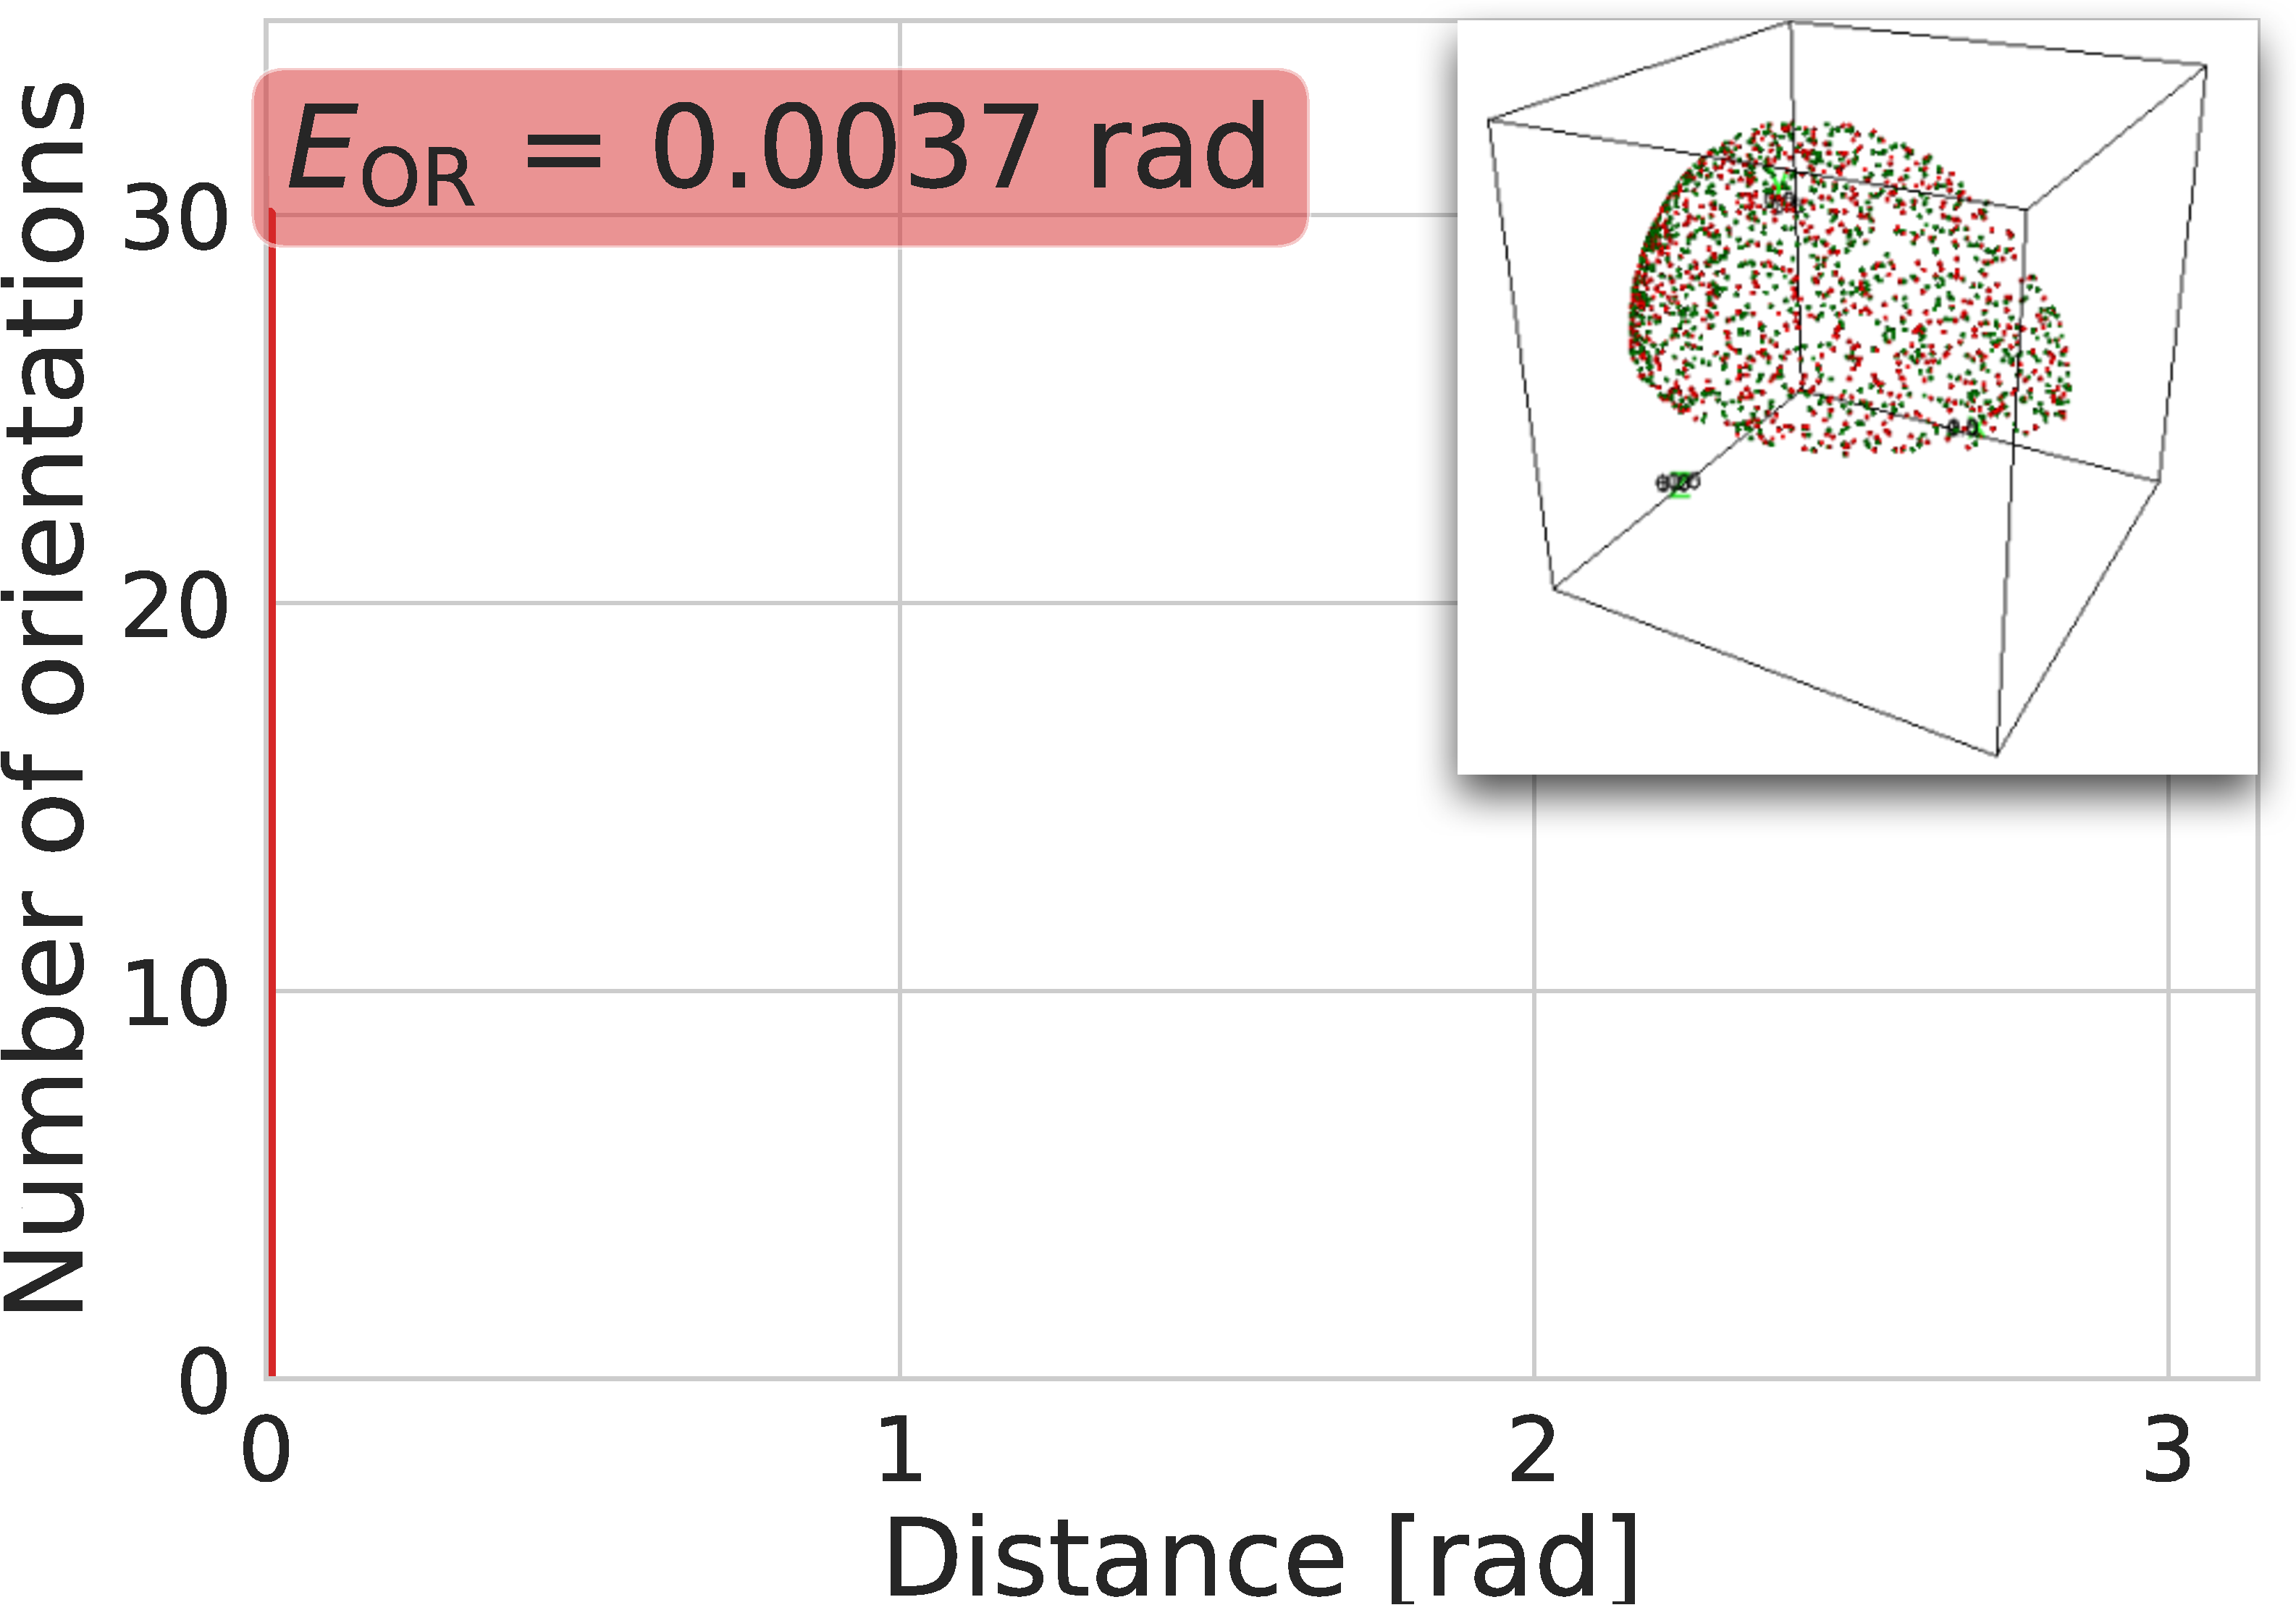
\includegraphics[height=3cm]{figures/AfterAA.pdf}
            \caption{Orientations after alignment.}
        \end{subfigure}
        \caption{%
            Example of perfect alignment~\eqnref{orientation-recovery-error} after a perfect orientation recovery~\eqnref{orientation-recovery}.
            The alignment error with corresponding directions $(\theta_2, \theta_1)$ before (a) and after (b) alignment.
            % and $\T$ as the optimum of \eqnref{orientation-recovery-error} on the right.
            %(b-c)~show the orientations projected on $\mathbb{S}^2 \subset \SO(3)$ before (b) and after (c) alignment.
            Green points are the true orientations $\{q_i\}$ and red points are the recovered orientations $\{\widehat{q_i}\}$.
            % The Figure (b) is exactly aligned which can be seen when zoomed. Due to plotting artifacts,
            While both colors are seen in (b), they are exactly superimposed.
        }\label{fig:5j0n-aa-loss-perfect-distances}
    %    \label{fig:angle-alignment-perfect}
    \end{minipage}
\end{figure}

\section{Euclidean distance between projections}\label{apx:results:distance-estimation}
% Orientation distance as, Estimating distances with

%\mdeff{Story: simplest baseline estimator, $d_{pe}$ somewhat estimates $d_q$, quickly plateaus (even in the simplest noiseless and centered case).
%Note the difference between symmetric and asymmetric proteins.}

\todo{Copy-edit.}

We evaluate $d_p(\p_i, \p_j) = \Vert \p_i - \p_j \Vert_2$ (\ie, the Euclidean distance) as a baseline distance estimator.
From $P = 5,000$ possible projection, we randomly select $5$ projections.
For each of these projections, we compute the Euclidean distance between aforementioned projection and all the others $d_p(\mathbf{p}_i,\mathbf{p}_j)=\lVert\mathbf{p}_i-\mathbf{p}_j\rVert_2$ and their corresponding orientation distance $d_q(q_i,q_j)$ through~\eqnref{distance:orientations}.
We then report the $(d_q,d_p)$ relationship for all pairs in \figref{euclidean-not-robust}, for both the \texttt{5j0n} (left) and \texttt{5a1a} (right).

Two principal observations can be made from this experiment.
First, as suspected, $d_p$ fails to be a consistent predictor of $d_q$, even in the simple imaging conditions considered here (no noise, no shift, no PSF).
In particular, the larger the quaternion distance $d_q$, the poorer the predictive ability of $d_p$ (the plot plateaus).
The other interesting observation is that the trend of $(d_q,d_p)$ plot of the \texttt{5a1a} appears to take symmetric shape of letter \texttt{M} which can be explained with the fact that this protein has intrinsic dihedral (D2) symmetry~\cite{noauthor_d2sym_nodate,noauthor_5a1asym_nodate}.
\mdeff{Check these refs. Other ones are used in main text?}

\begin{figure}[ht!]
    \begin{minipage}[t]{0.57\linewidth}
        \begin{subfigure}[t]{0.48\textwidth}
            \centering
            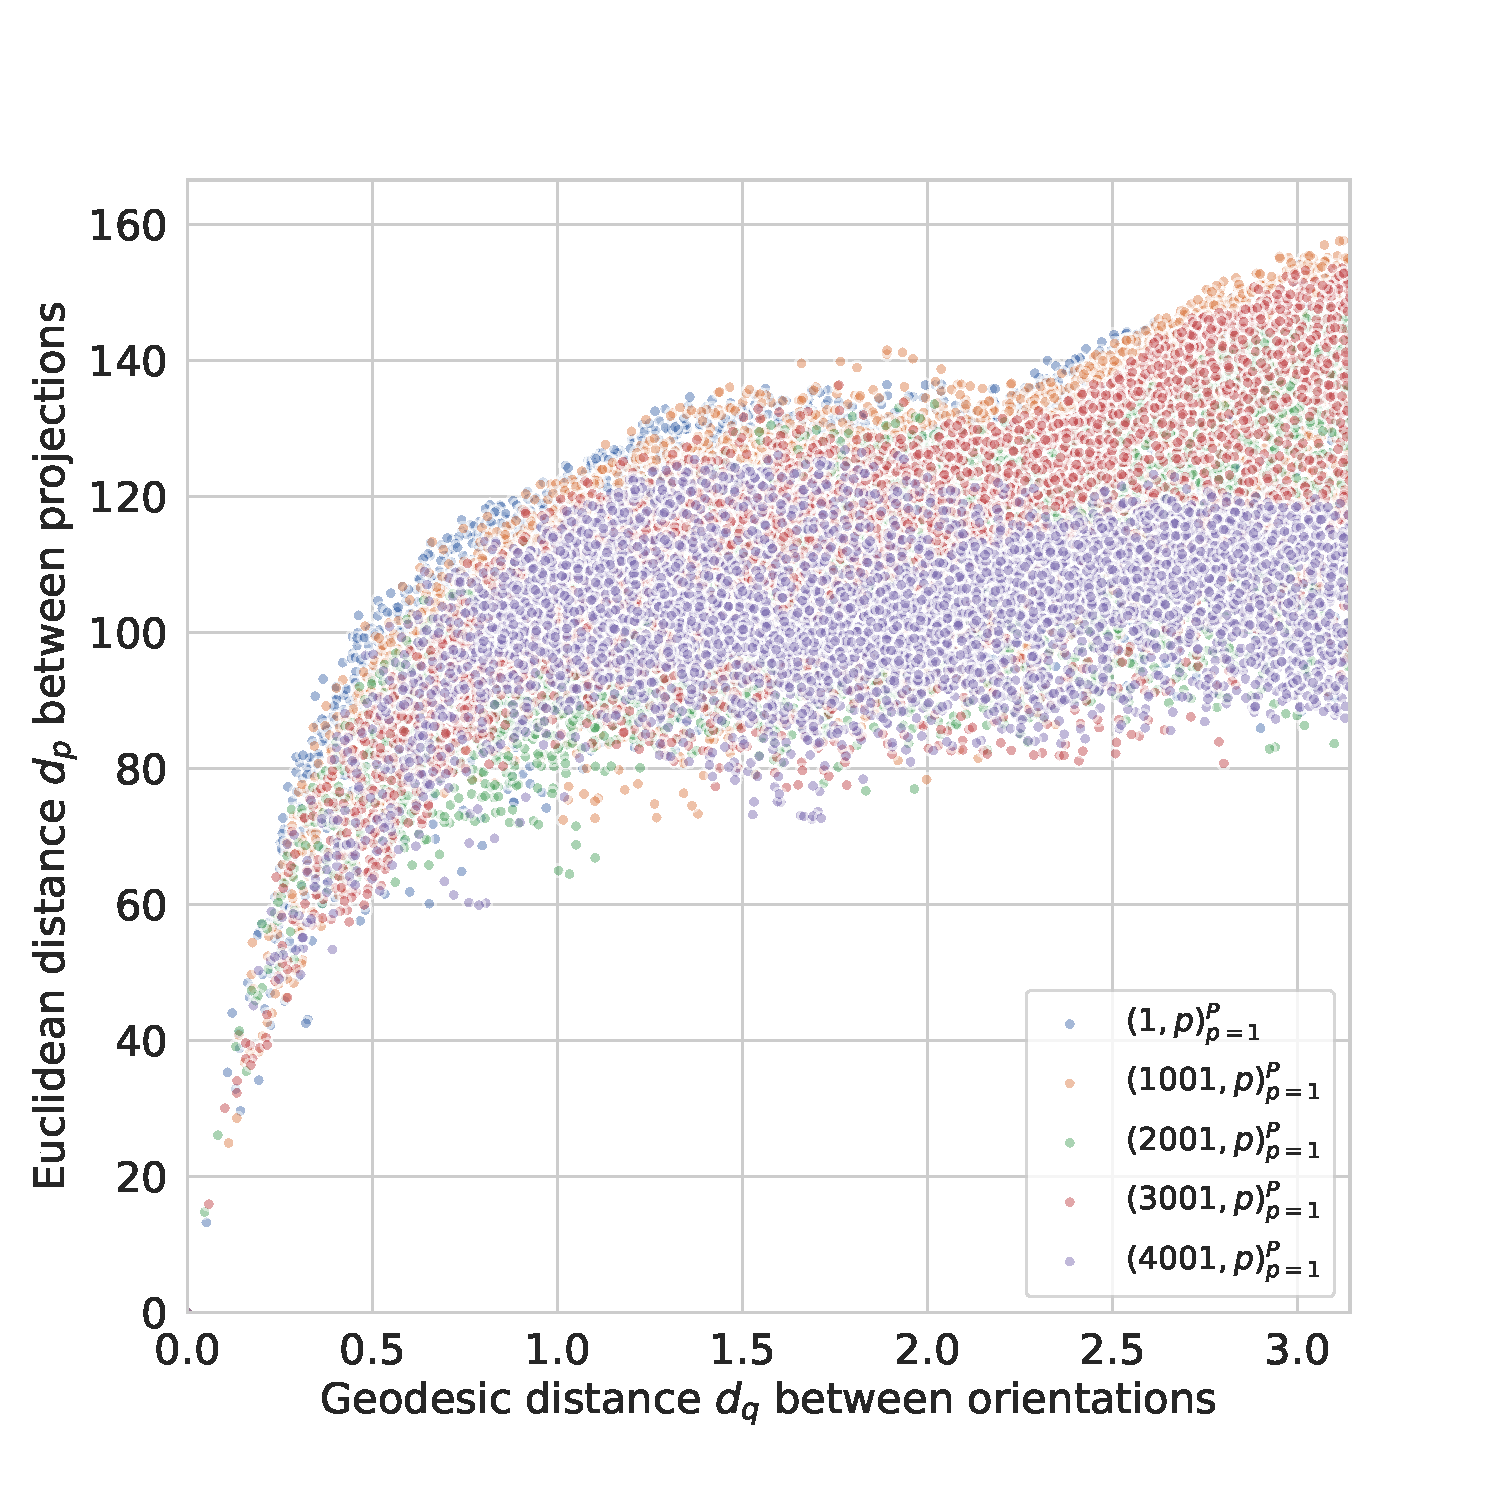
\includegraphics[height=4cm]{figures/eucl_notrobust_5j0n}
            \caption{\texttt{5j0n}}
        \end{subfigure}
        \hfill
        \begin{subfigure}[t]{0.48\textwidth}
            \centering
            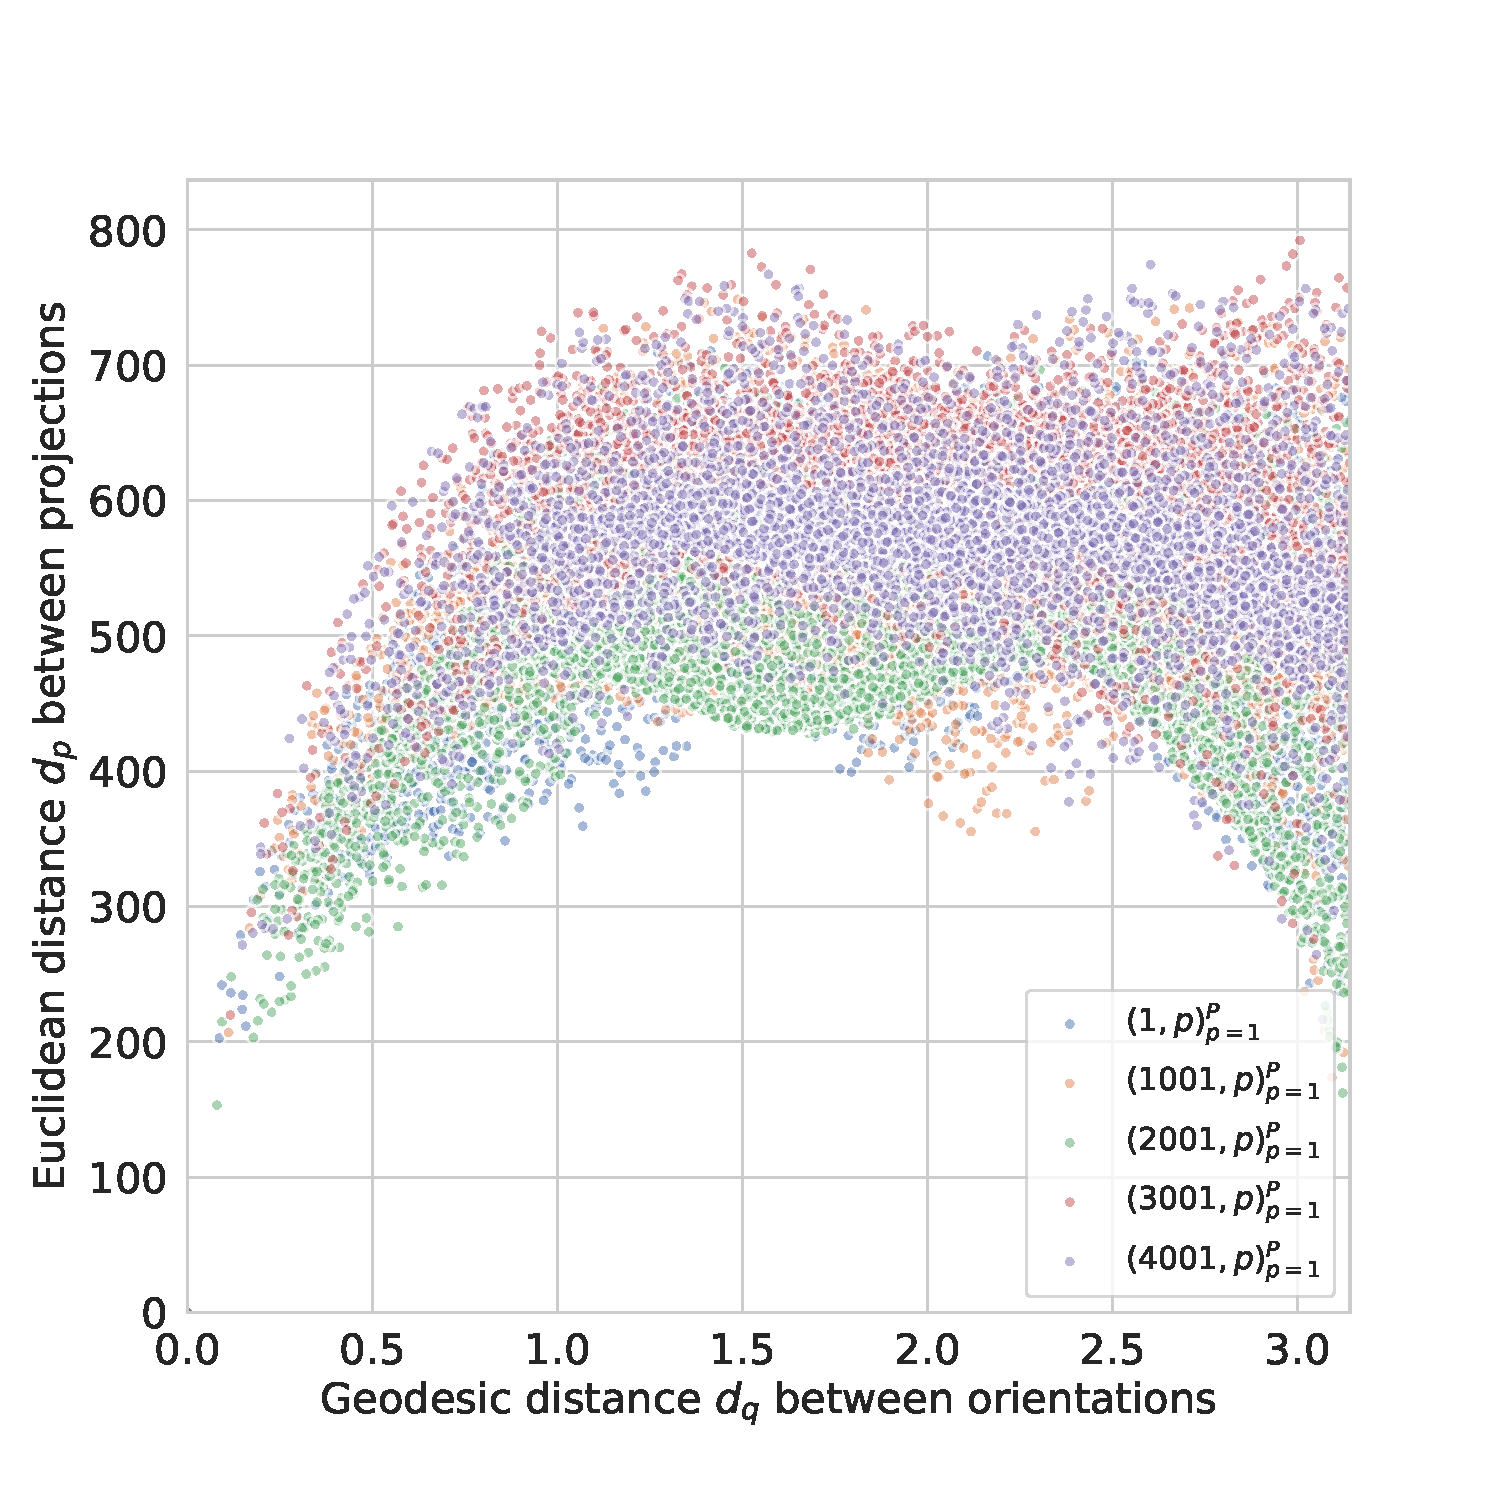
\includegraphics[height=4cm]{figures/eucl_notrobust_5a1a}
            \caption{\texttt{5a1a}}\label{fig:euclidean-not-robust:5a1a}
        \end{subfigure}
        \caption{%
            The Euclidean distance between two projections $d_p(\p_i, \p_j) = \Vert \p_i - \p_j \Vert_2$ versus their actual relative orientation $d_q(q_i, q_j)$ with the half-sphere direction coverage.
            Each color represent the distances between one fixed projection and the other $P-1$ projections.
    %        The color corresponds to projection pairs that share one projection, \ie, distance between one projection with all other projections.
            While there is some correlation, especially at small distances, the Euclidean distance is a poor estimator.
            Because \texttt{5a1a} has D2 symmetries, two projections might be identical while not having been acquired from the same orientation.
            \mdeff{Is there a reason (other than historical) for those dPdQ plots to be different (w.r.t.\ how distances are sampled) from the ones in \figref{distance-learning:dpdq} and \figref{geo-eucl-mlp}?}
        }\label{fig:euclidean-not-robust}
    \end{minipage}
\end{figure}

\section{Estimating distances on unseen proteins}\label{apx:unseen-proteins}
%\section{Non-determinism of the Orientation Recovery}\label{apx:non-determinism}

As the SiameseNN will ultimately be trained on known proteins and used to estimate distances on unknown proteins to be imaged,
%we also desire our learned distance function to generalize/transfer across density maps $\x$.
we also desire our learned distance function to generalize to unseen proteins.
The distance function $\widehat{d_p}$ must abstract the protein---in the same way it must abstract shifts, noise, or PSFs to generalize to unseen projections.
We attempted to recover the orientations of noiseless projections from \texttt{5j0n} while we had trained the SiameseNN on $4,000$ noiseless projections from four other proteins (\texttt{5nvu}~\cite{ZHANG20171303}, \texttt{5nvs}~\cite{ZHANG20171303}, \texttt{6mem}~\cite{iwai2018unique}, \texttt{6o1o}~\cite{liu2019target}, which have the same type of symmetry as \texttt{5j0n}).
%In this experiment, we generated $1,000$ projections per protein.
%\todo{should be the same ``kind'' of refs as the ones used in 3.1 for \texttt{5j0n} and \texttt{5a1a}}
%Four proteins were used in the training and validation set to ensure the robustness to the unseen protein \texttt{5j0n} used in the testing set.
%The number of projections in every set is the same as in \tabref{dataset}.
We obtained a recovery loss of \todo{$L_\text{OR} = 0.0352$},
to be compared with \todo{$L_\text{OR} \approx 0.11$} when the SiameseNN was trained on \texttt{5j0n} alone.
While performance is somewhat degraded, we conclude that it is possible to train and use a distance function on different proteins.

\todo{Distance learning and orientation recovery worked well, but alignment didn't.}
\mdeff{Why is dPdQ so bad? Seems contradictory to a low $L_\text{DE}$ and $L_\text{OR}$. Maybe that's why alignment didn't work? But then I don't get why $L_\text{DE}$ and $L_\text{OR}$ are so low\ldots.}

\mdeff{Could we also have $E_\text{OR}$? It's easier to understand and compare.}
\banjac{I fully agree, however, I already mentioned that I wasn't able to align the orientations even though the $L_\text{OR}$ was very good. Looking at the estimation and GT in rotation space, it is visible we have some kind of transformation between these two (transformation similar to one we found the flip is causing, but it is not the flip).}
\mdeff{Could we show the ground-truth and estimated orientations in \figref{robustness-to-unseen-pipeline}?}

While alignment is in principle only necessary to compute $E_\text{OR}$, for an unknown reason, we had to align the recovered orientations with \eqnref{orientation-recovery-error} before feeding them to ASTRA\@.
\banjac{Hypothesis: I think ASTRA tools for reconstruction have one coordinate system and our protein is reconstructed in another. The alignment that we do as a last step of the pipeline is actually the alignment to ASTRA coordinate system. I am not sure if modifying}

\begin{figure}[ht!]
    \centering
    \begin{subfigure}[b]{0.35\linewidth}
        \centering
        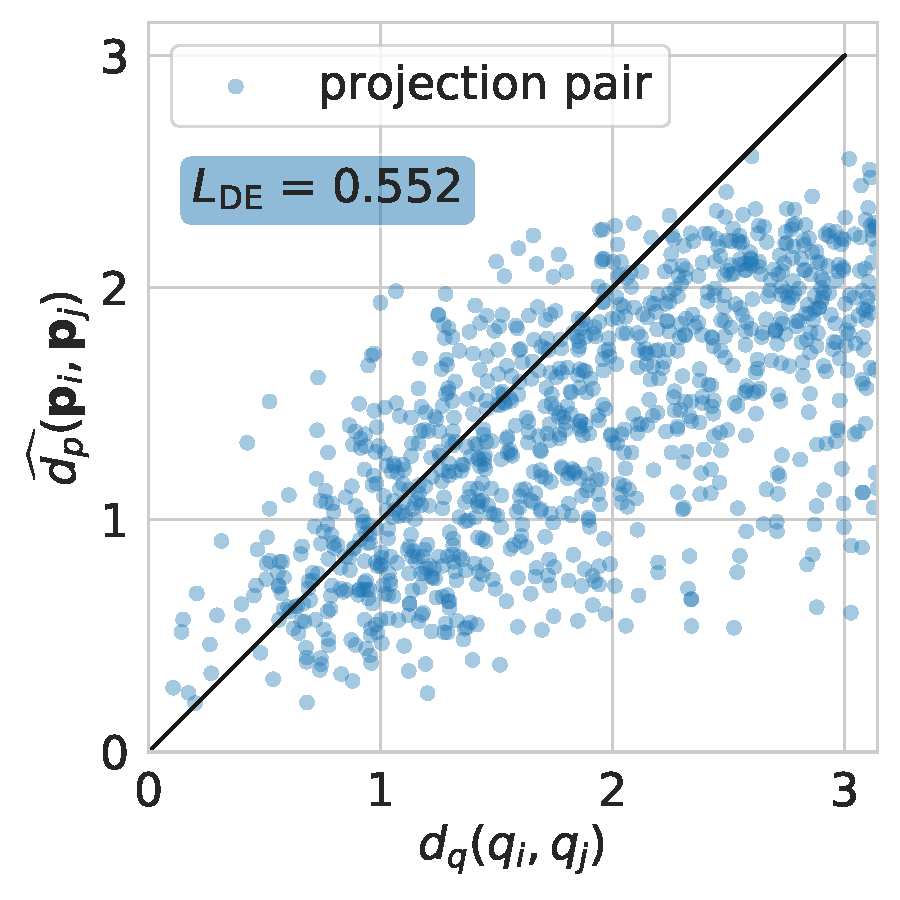
\includegraphics[height=4cm]{figures/dPdQ_5j0n_robustness_to_unseen.pdf}
        \caption{Relationship between $\widehat{d_p}$ and $d_q$ on $1,000$ pairs sampled from the test set of \texttt{5j0n}.}
    \end{subfigure}
    \hfill
    \begin{subfigure}[b]{0.60\linewidth}
        \centering
        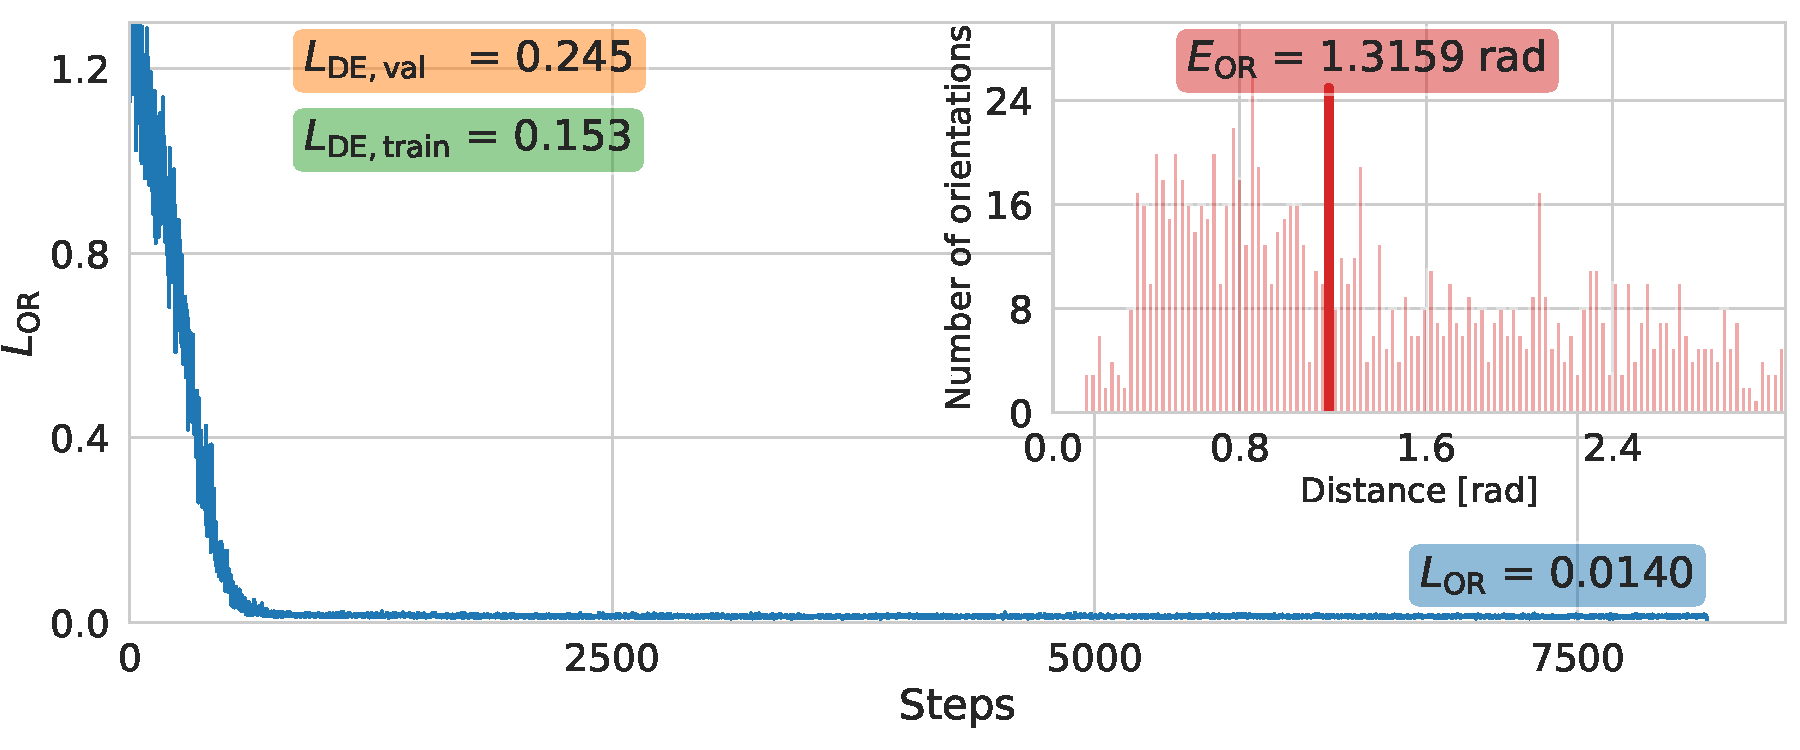
\includegraphics[height=4cm]{figures/5j0n_ar_aa_robustness_to_unseen.pdf}
        \caption{Recovered $\{ \widehat{q_i} \}$ from noiseless \texttt{5j0n} projections $\{ \p_i \}$ from protein unseen from distance estimation algorithm.}
    \end{subfigure}
    \caption{%
        Robustness to unseen protein \texttt{5j0n} pipeline results.
    }\label{fig:robustness-to-unseen-pipeline}
\end{figure}

\section{SiameseNN: feature distance}\label{apx:siamese:feature-distance}

%\mdeff{Story: $d_f = d_q$ better than Euclidean and MLP $d_f$. }

There are multiple options for a distance function $d_f$ between two features $\mathbf{f}_i = \mathcal{G}_w(\p_i) \in \R^{n_f}$.
\figref{geo-eucl-mlp} compares the use of the Euclidean distance $d_f(\f_i, \f_j) = \Vert \f_i - \f_j \Vert_2$ and the cosine distance $d_f(\f_i, \f_j) = 2 \arccos \left( \frac{\langle \f_i, \f_j \rangle}{\lVert \f_i \rVert \lVert \f_j \rVert} \right)$: The cosine distance results in a lower $L_\text{DE}$, which makes $\widehat{d_p}$ a better estimator of $d_q$.
% the projection pairs deviate the least from the identity
This superiority of the cosine distance is likely due to its capacity to model the elliptic geometry of $\SO(3)$, a feat the Euclidean distance does not achieve, the Euclidean space being neither periodic nor curved.
%The $\SO(3)$ is non-linear and it can be explained with the fact that Euclidean distance of two quaternions can be small, despite the rotation being large~\cite{huynh_metrics_2009,DBLP:journals/corr/abs-1805-01026}.
We also tried to parametrize $d_f$ as a multi-layer perceptron (MLP) but were unable to train it.

% The MLP we tested was made of six layers with $1024, 512, 512, 256, 256, 1$ units, all of which use the SeLU activation function.
% The features $\f_i$ and $\f_j$ were stacked as an array of size $2n_f$ before being fed to the MLP\@.
% Note that, while a MLP can approximate any function, there is no guarantee that the learned function will satisfy the axioms of a proper distance function (\ie, the identity of indiscernibles, symmetry, and triangle inequality).

\begin{figure}[ht]
    \centering
    \begin{subfigure}[b]{0.49\linewidth}
        \centering
        % 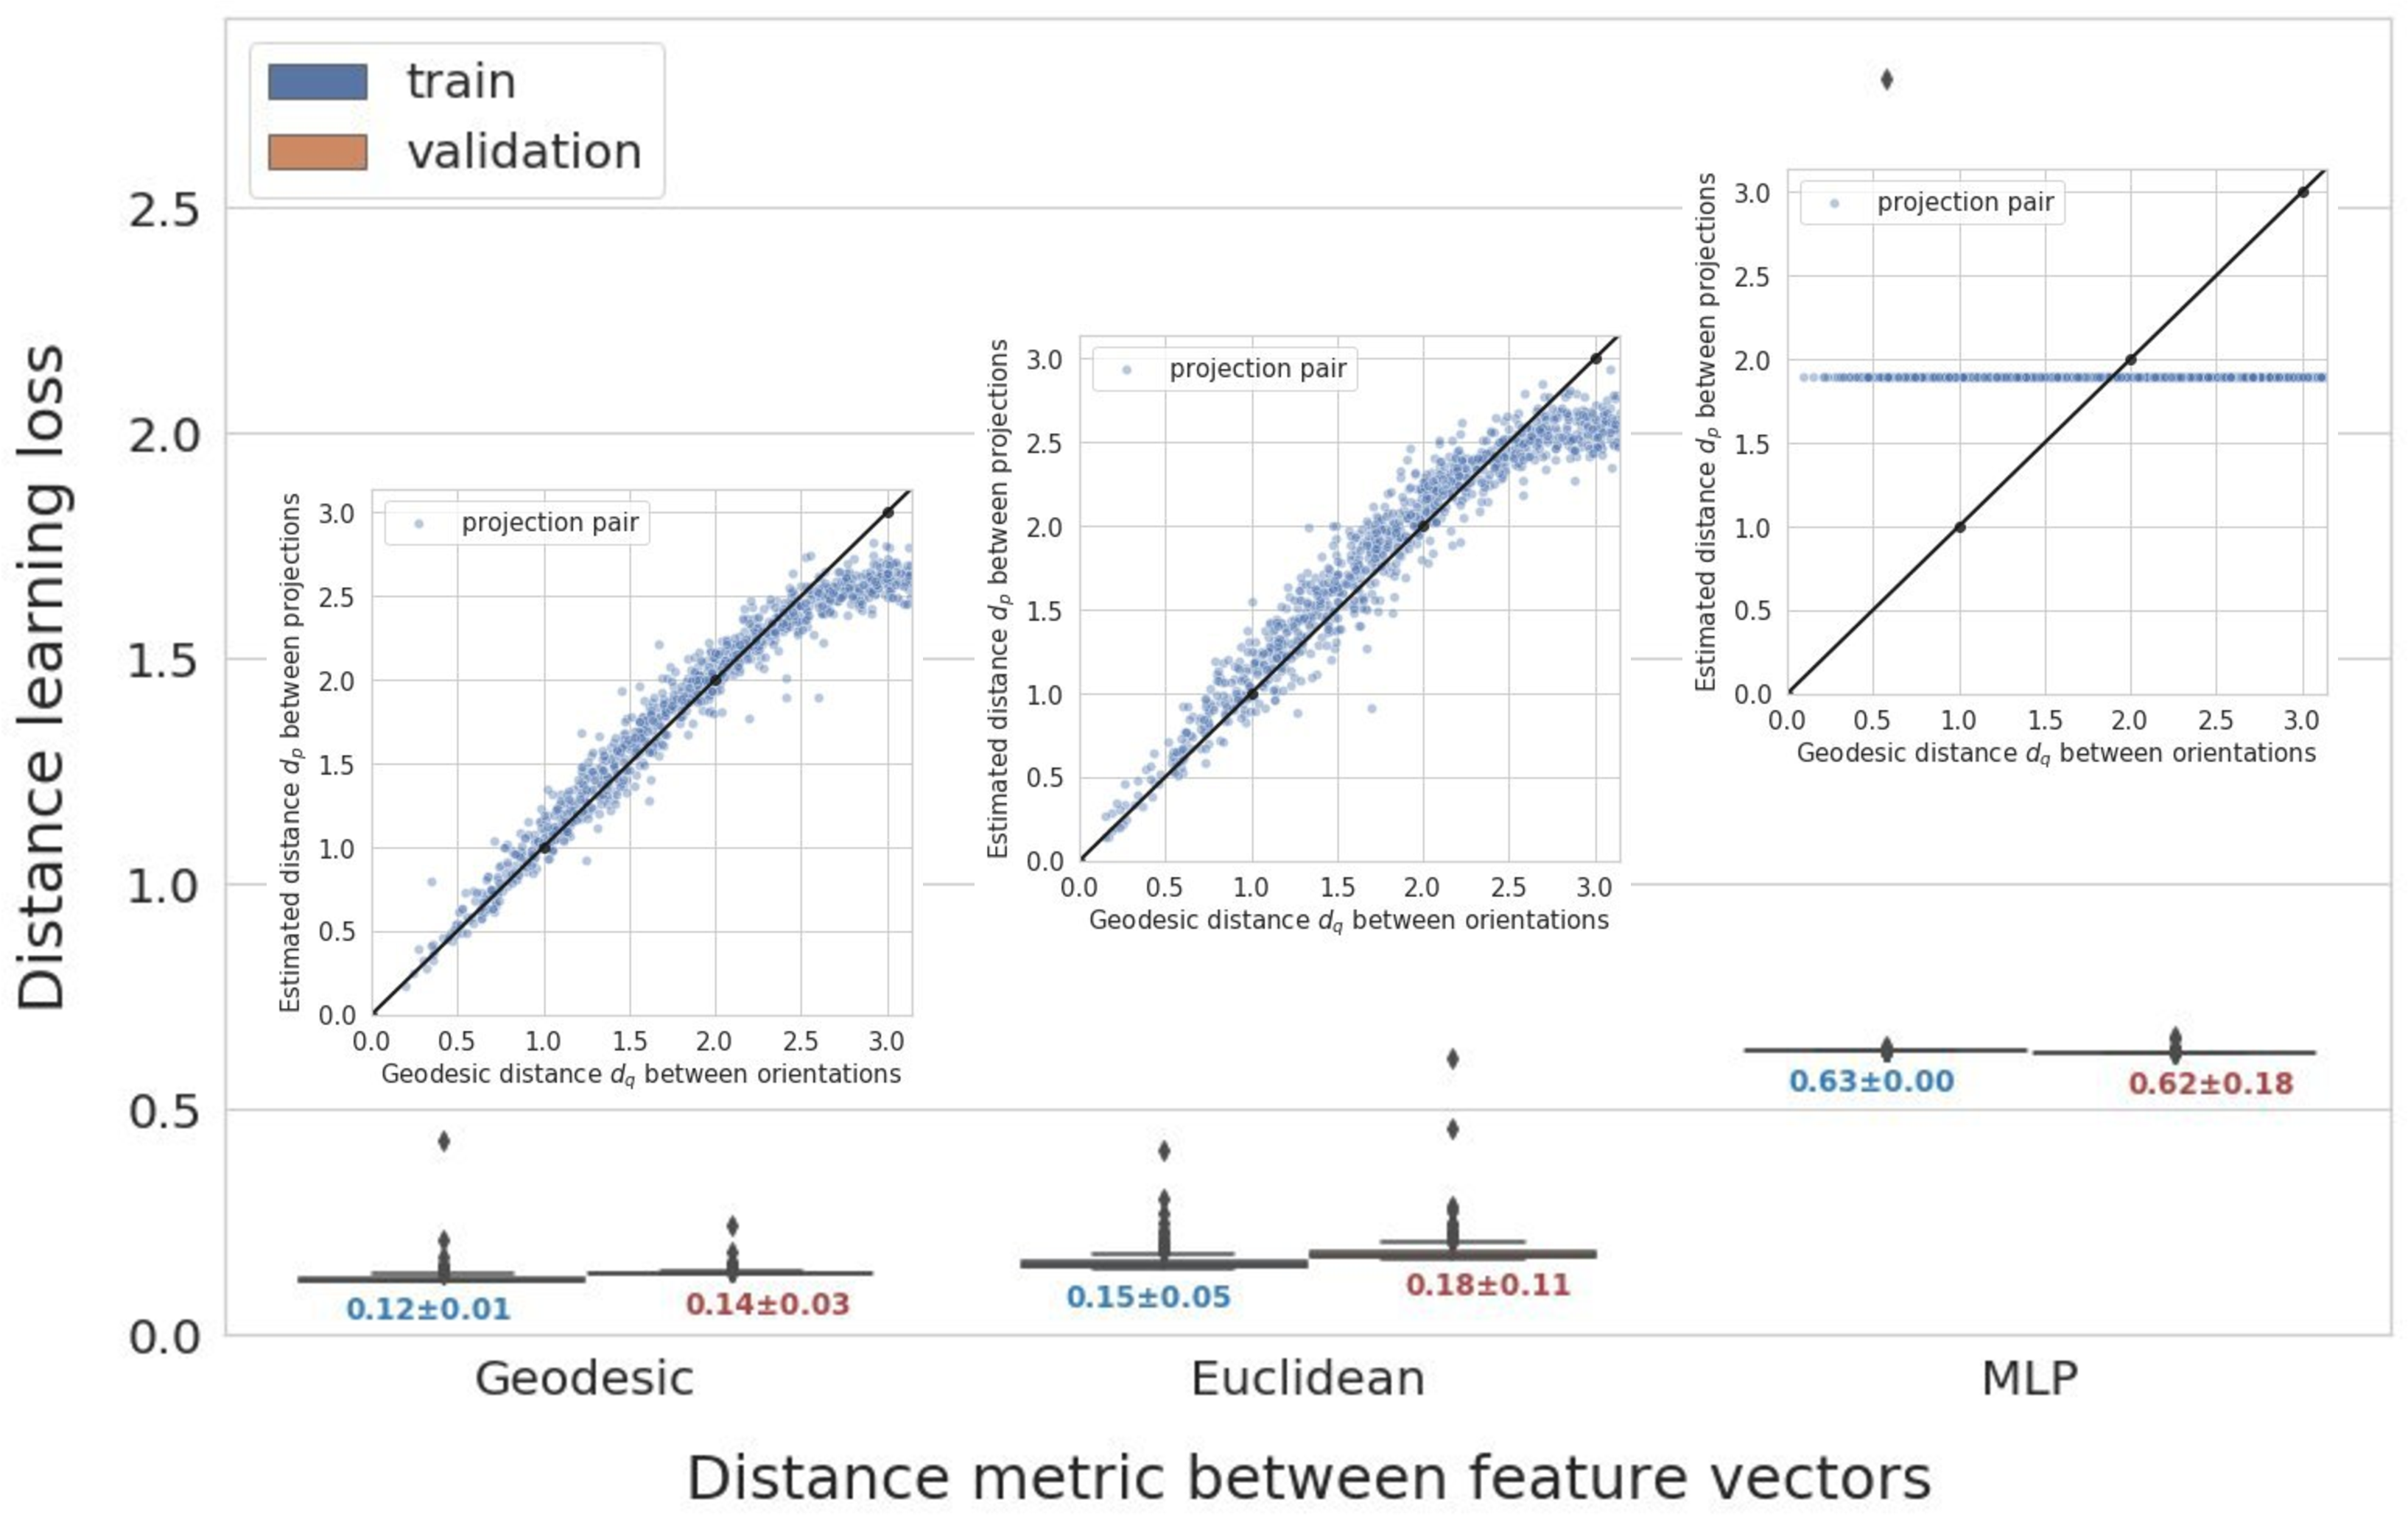
\includegraphics[height=4cm]{figures/geo_eucl_mlp_distance_metric.pdf}
        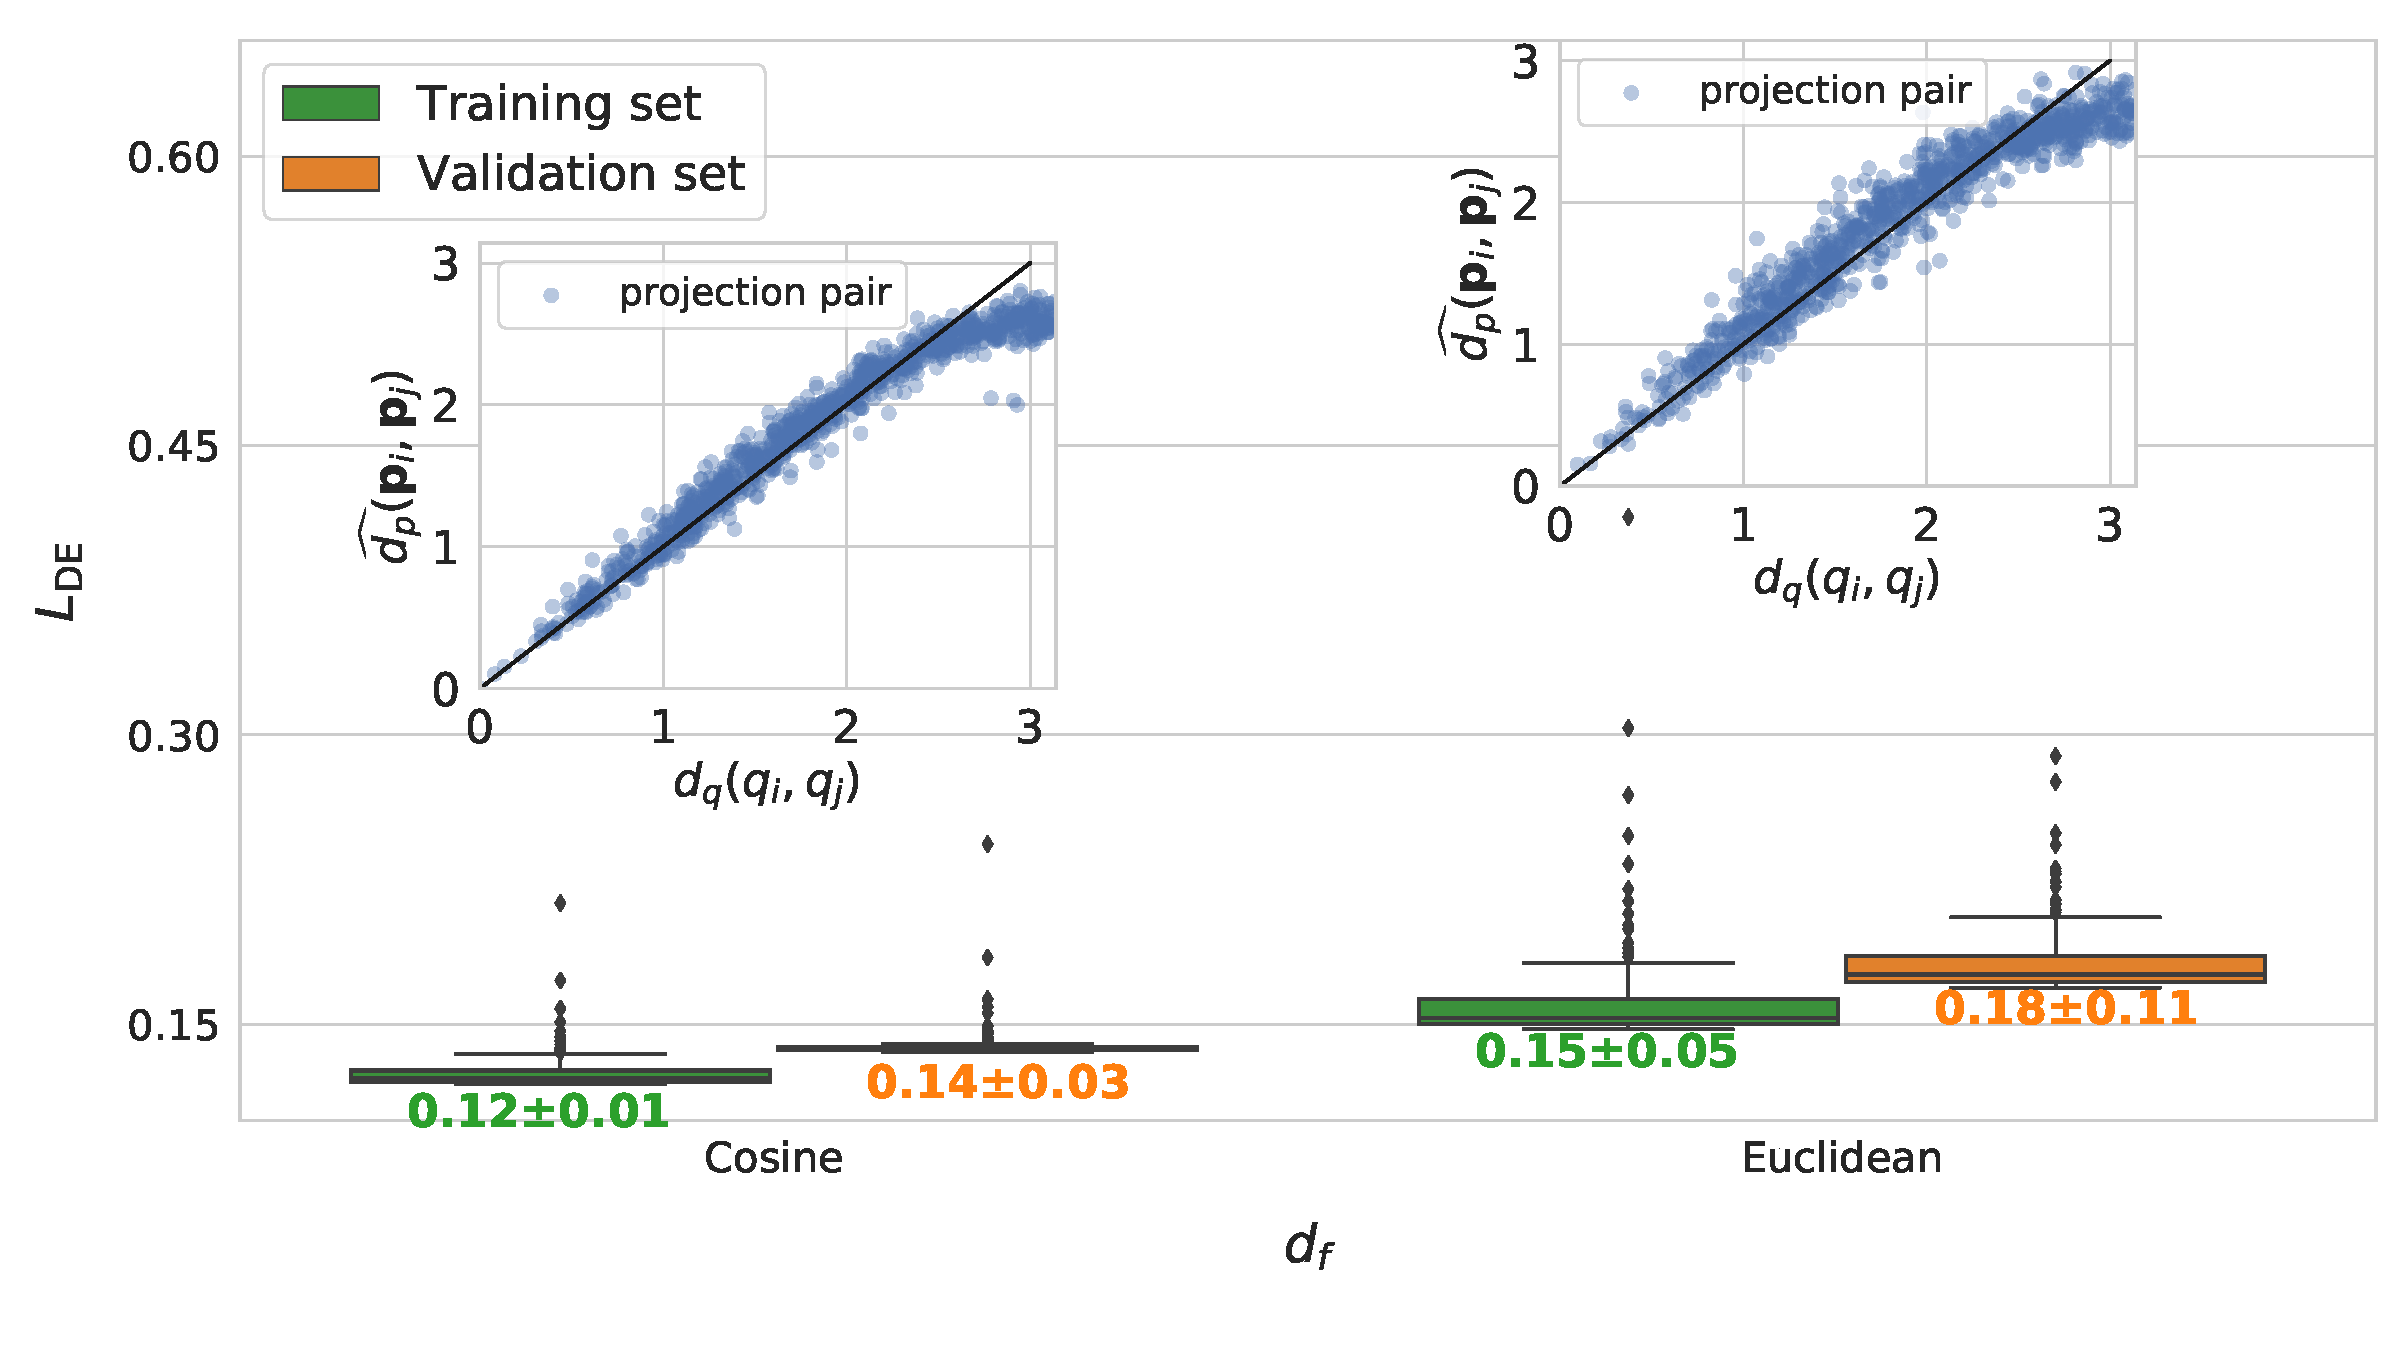
\includegraphics[height=4cm]{figures/dPdQ_feat_distances.pdf}
        \caption{%
            Performance of distance learning w.r.t.\ the choice of feature distance function $d_f$.
            The box plots show the distance learning loss $L_\text{DE}$ \eqnref{distance-learning}.
            The inserted plots show the relationship between $d_p(\p_i, \p_j) = d_f(\mathcal{G}_w(\p_i), \mathcal{G}_w(\p_j))$ and $d_q(q_i, q_j)$.
            %\mdeff{It might be clearer (also for the caption) to move the inserted plots out and show them separately on the right (in places of the ones that are there now).}
        }\label{fig:geo-eucl-mlp}
    \end{subfigure}
    \hfill
    \begin{subfigure}[b]{0.48\linewidth}
        \begin{subfigure}[t]{0.48\linewidth}
            \centering
            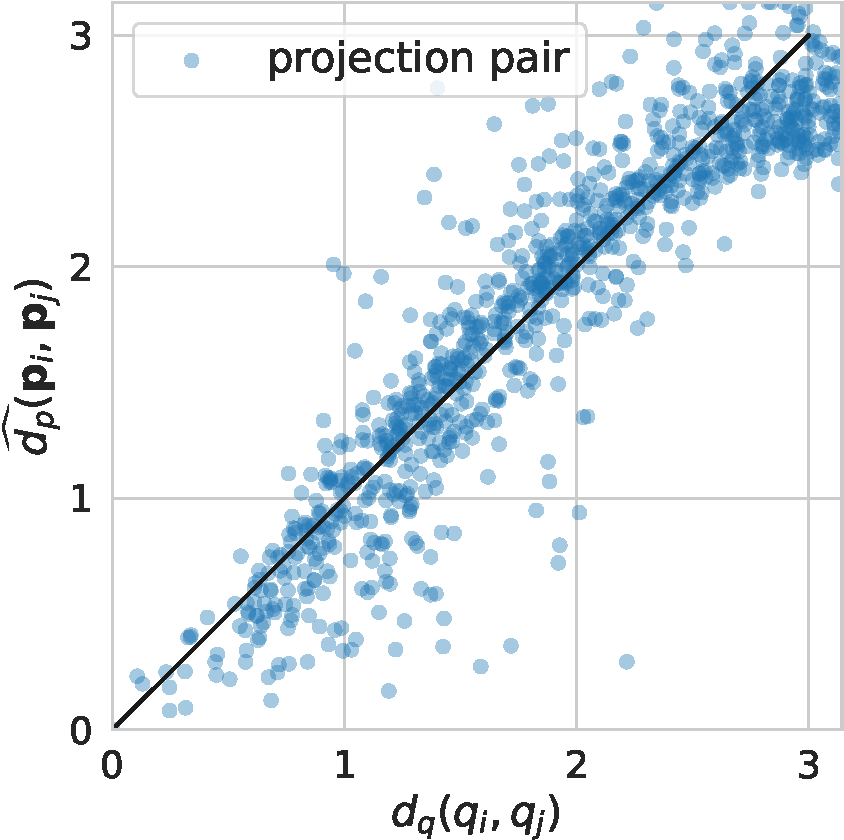
\includegraphics[height=3.5cm]{figures/dPdQ_5j0n_4d.pdf}
            \caption*{$n_f=4$} % and half-directions.
        \end{subfigure}
        \hfill
        \begin{subfigure}[t]{0.48\linewidth}
            \centering
            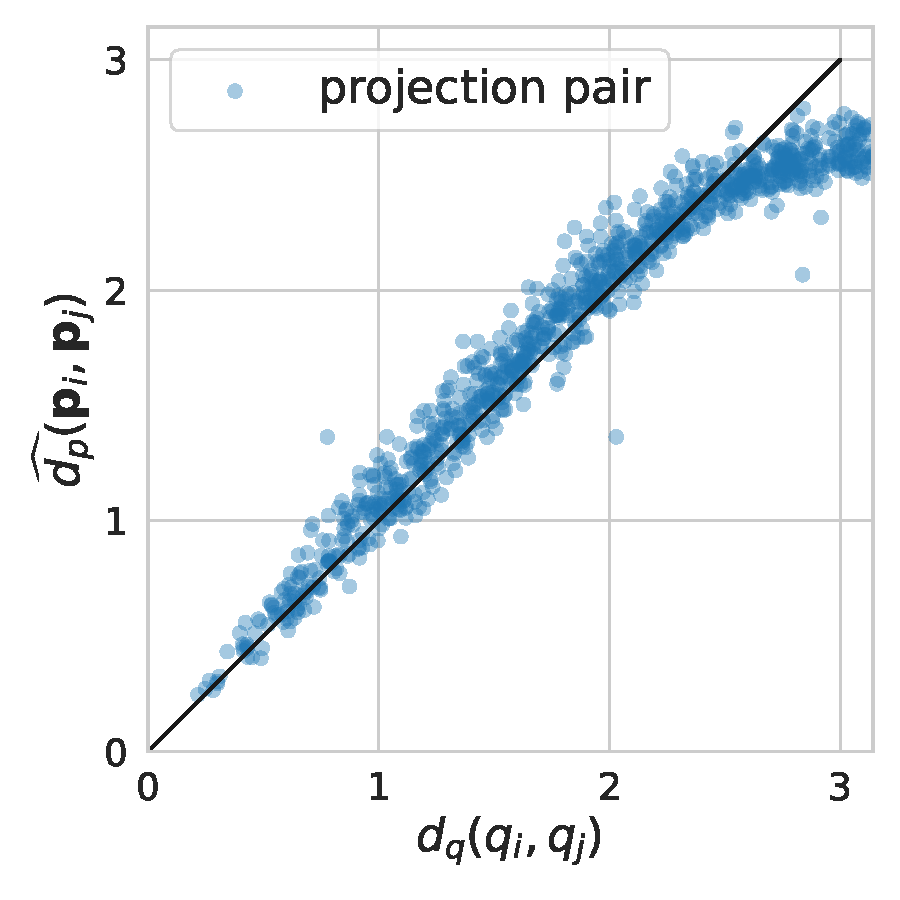
\includegraphics[height=3.5cm]{figures/dPdQ_5j0n_256.pdf}
            \caption*{$n_f=256$} % and half-directions.
        \end{subfigure}
        % \hfill
        % \begin{subfigure}[t]{0.31\linewidth}
        %     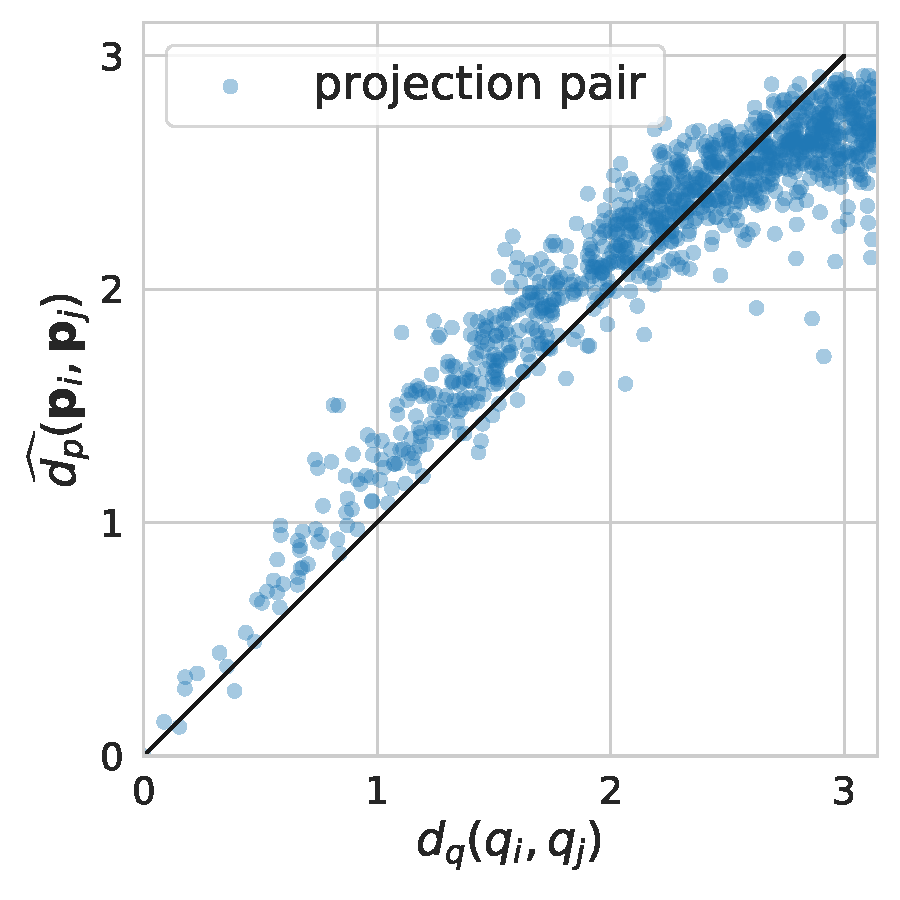
\includegraphics[width=\linewidth]{figures/dPdQ_5j0n_full.pdf}
        %     \caption{$n_f=256$ and all-directions.}
        % \end{subfigure}
        \caption{%
            Performance of distance learning w.r.t.\ the choice of embedding dimensionality $n_f$.
            Relationship between $\widehat{d_p}$ and $d_q$ on $1,000$ pairs sampled from the test set of \texttt{5j0n}.
            \mdeff{Might be interesting to show other choices for $n_f$. There will probably be a trend of increasing performance with diminishing returns.}
            %Different direction constrains in \figref{orientation-constraints}.
        }\label{fig:4d-vs-256d-de}
    \end{subfigure}
        \caption{%
            Performance of distance learning w.r.t.\ the choice of feature distance function $d_f$ (a) and of embedding dimensionality $n_f$ (b).
            \mdeff{Both figures should be similar as they show the same thing: performance w.r.t.\ the choice of an hyper-parameter ($d_f$ and $n_f$). Do we have $L_\text{DE}$ for the two $n_f$?}
        }
\end{figure}

\section{SiameseNN: embedding dimension}\label{apx:siamese:embedding-dimension}

\mdeff{Merge \apxref{siamese:feature-distance} and \apxref{siamese:embedding-dimension} as a single appendix discussing SiameseNN (feature space) hyper-parameters?}

\figref{4d-vs-256d-de} shows the performance of our distance estimator $\widehat{d_p}$ depending on the size of embedding space $n_f$.
It clearly indicates that a space of $n_f=4$ dimensions is insufficient to represent the complexity/variability of projections.
% $n_f=4$ dimensional space is too constrained
That is a motivation to embed the projections in a space of higher dimensions that can represent more variation than the orientation, and abstract that variation by solely considering the distances between the embedded projections $\f_i = \G_w(\p_i)$.
%Great motivation for our indirect method and $n_f>4$, even when trained and tested on the same protein.

%Difference in the architecture of networks with $n_f=4$ or $n_f=256$ is in \apxref{siamese-architecture}.

%\clearpage
\section{SiameseNN architecture}\label{apx:siamese-architecture}

\begin{figure}[ht!]
    \centering
    \begin{subfigure}[t]{0.5\linewidth}
        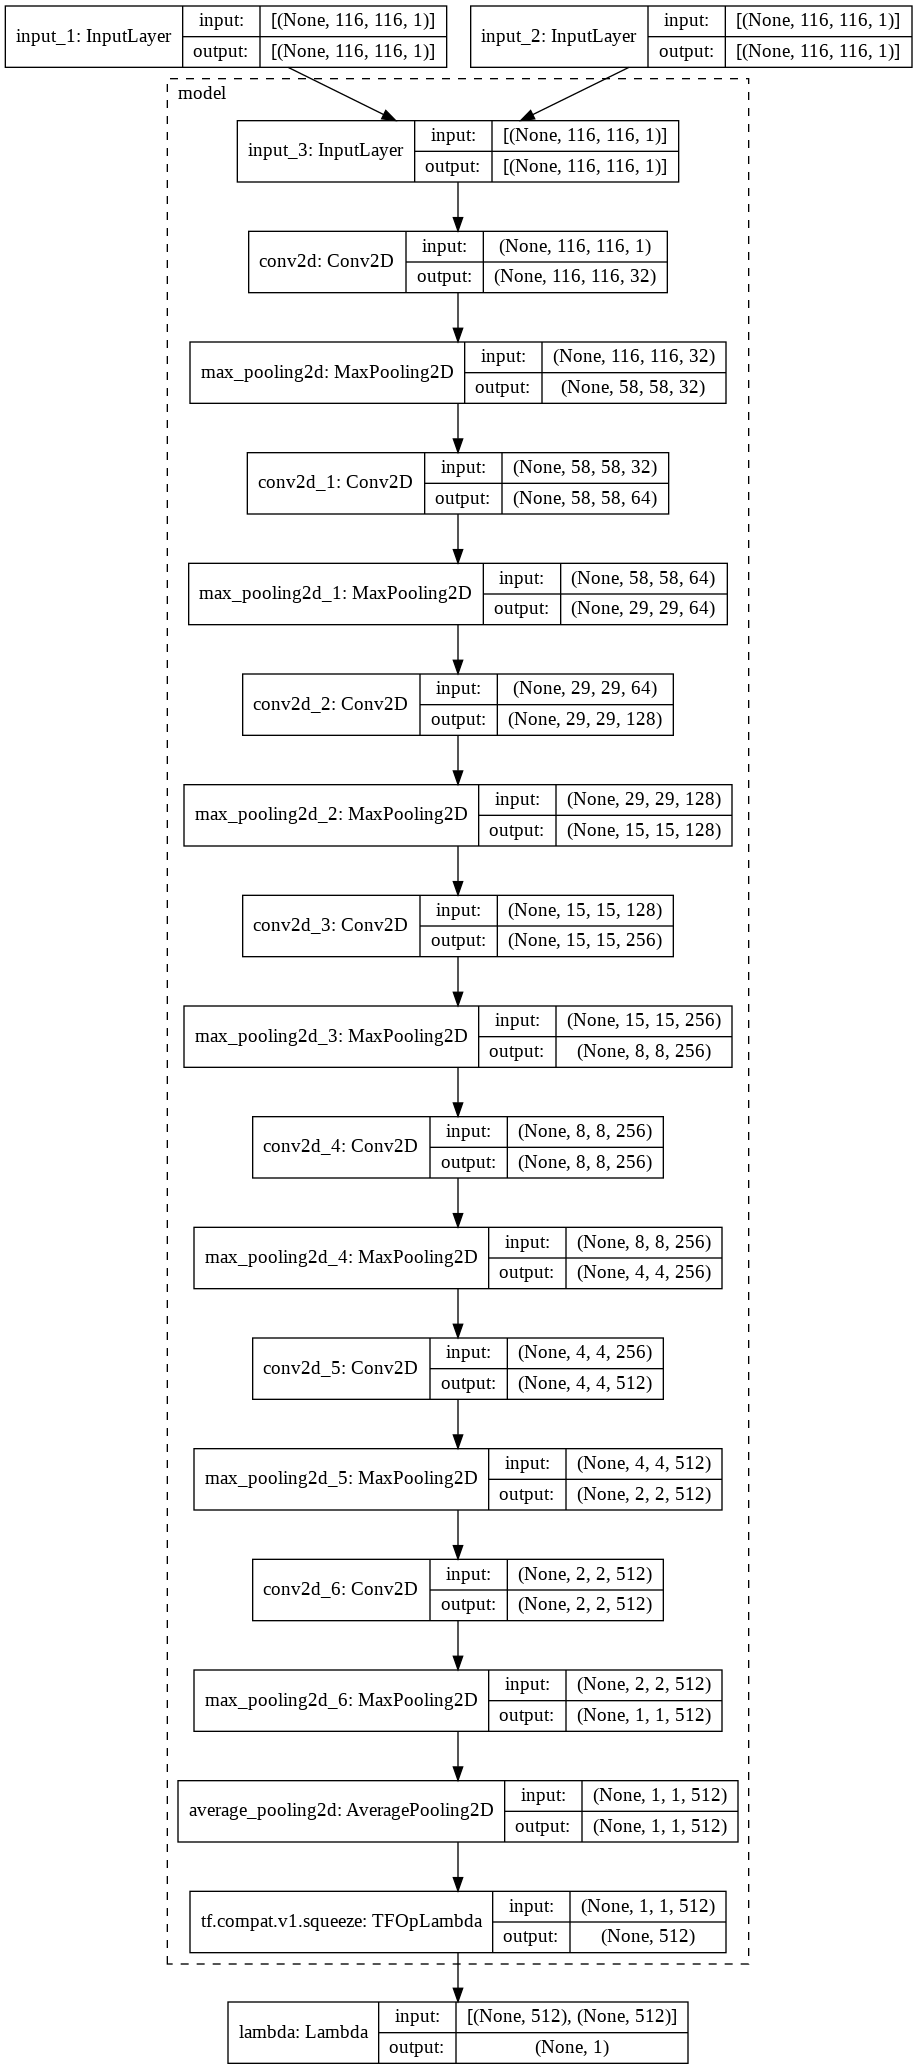
\includegraphics[width=\linewidth]{figures/model_plot_256d.png}
    \end{subfigure}
    \caption{%
        Distance estimation network architecture.
        We have two input images of dimensions $116 \times 116$.
        Each one goes to its CNN (part where we share the weights, selected with a dashed line).
        The output is a scalar value representing the distance between these two images.
        Last layer converts feature vector to a higher-dimensional vector of size $n_f=256$. This architecture of network was used throughout all experiments. The last layer was different for $n_f=4$.
        \mdeff{Would be easier to only show the CNN $\G_w$, say that an image $\p \in \R^{n_p}$ (with $n_p = 116 \times 116$ for \texttt{5j0n} and $275 \times 275$ for \texttt{5a1a}) goes in and a feature $\f \in \R^{n_f}$ ($n_f=256$) goes out.}
        \mdeff{Why is the last layer 512 dimensions if $n_f=256$?}
        \mdeff{The \texttt{average\_pooling} is here to make $\G_w$ agnostic to the image size right? We should explain that. Maybe show two models as two columns, one with input $116 \times 116$ and the other with $275 \times 275$? Or instead of numbers, write $\lceil \sqrt{n_p}/2 \rceil$, $\lceil \sqrt{n_p}/4 \rceil$, etc.?}
        \mdeff{Also the batch size could be made more explicit than \texttt{None}.}
        \mdeff{Make the figure smaller: don't repeat every sizes as input and output. Try a more horizontal aspect ratio?}
        \mdeff{The size of the convolutional filters (\eg, $3 \times 3$) are missing.}
    }\label{fig:de-architecture}
\end{figure}
